\documentclass[12pt]{article}
\usepackage{amsmath,amsfonts,nicefrac}
\usepackage{graphicx}
\usepackage{enumerate}
\usepackage{natbib}
\usepackage{url} % not crucial - just used below for the URL 
\usepackage{ifthen}

%\pdfminorversion=4
% NOTE: To produce blinded version, replace "0" with "1" below.
\newcommand{\blind}{1}
% DON'T change margins - should be 1 inch all around.
%\addtolength{\oddsidemargin}{-.5in}%
%\addtolength{\evensidemargin}{-.5in}%
%\addtolength{\textwidth}{1in}%
%\addtolength{\textheight}{-.3in}%
%\addtolength{\topmargin}{-.8in}%

\usepackage[margin=0.5in]{geometry}
\usepackage[table]{xcolor}% http://ctan.org/pkg/xcolor

\newcommand{\cl}[2]{\cellcolor{#1!#2}}
\newcommand{\inc}[2]{ \ifthenelse{\equal{#1}{1}}{\input{./sections/#2}}{ } }



\begin{document}

%\bibliographystyle{natbib}

\def\spacingset#1{\renewcommand{\baselinestretch}%
{#1}\small\normalsize} \spacingset{1}


%%%%%%%%%%%%%%%%%%%%%%%%%%%%%%%%%%%%%%%%%%%%%%%%%%%%%%%%%%%%%%%%%%%%%%%%%%%%%%

\if1\blind
{
  \title{\bf Towards Structured Use of Bayesian Sequential Monitoring in Clinical Trials}
  \author{Evan Kwiatkowski\textsuperscript{$\dagger$}, 
	        Eugenio Andraca-Carrera\textsuperscript{$\ddagger$},\\
					Mat Soukup\textsuperscript{$\ddagger$},
					\medskip Matthew A. Psioda\textsuperscript{$\dagger$}\thanks{The authors gratefully acknowledge \textit{please remember to list all relevant funding sources in the unblinded version}}\\
	  %
	  $\dagger$ Department of Biostatistics,
		University of North Carolina, \\
		McGavran-Greenberg Hall, CB\#7420, \\
		%
		\medskip Chapel Hill, North Carolina, U.S.A.\\
    $\ddagger$ Division of Biometrics VII, Office of Biostatistics \\
		           Center for Drug Evaluation and Research, \\
							 US Food and Drug Administration, \\
							 Silver Spring, Maryland, USA \\									
		}
  \maketitle
} \fi

\if0\blind
{
  \bigskip
  \bigskip
  \bigskip
  \begin{center}
    {\LARGE\bf Title}
\end{center}
  \medskip
} \fi

\bigskip
\begin{abstract}
The text of your abstract. 200 or fewer words.
\end{abstract}

\noindent%
{\it Keywords:}  3 to 6 keywords, that do not appear in the title
\vfill

\newpage
\spacingset{1.5} % DON'T change the spacing!



\section{Introduction}

Things to discuss:
\begin{itemize}
 \item 21\textsuperscript{st} Century Cures Act (MATT)
 \item PDUFA VI reauthorization (MATT)
 \item Expansive work already done on sequential monitoring  (EVAN -- draft on 6/21)
%\item Berry A Case for Bayesianism, Cornfield The Bayesian outlook, classical arguments for Bayes in clinical trials, not sequential monitoring in particular
%\item (1) Berry Montoring Accumulating Data, (2) Cornfield/Greenhouse On certain aspects, (3) Cornfield Sequential Trials, (4) A Bayesian Test of Some Classical Hypotheses, with Applications to Sequential Clinical Trials Jerome Cornfield 
%\item Bayes \& monitoring, based on posterior distributions
%\item First papers in Bayes sequential monitoring. Bayesian inferences not affected by frequent or continual monitoring by the likelihood principle.
%\item Papers which compare to frequentist stopping rules \& increased interpretation on role of priors.
%\item \cite{Spiegelhalter1994}
%\item \cite{Spiegelhalter1993} predictive distributions as basis for monitoring
%\item \cite{Freedman1992} choice of prior explained by showing its impact on percentiles of posterior distribution
%\item \cite{Freedman1989} The need to overcome this `\textbf{handicap}' prevents unduly early termination.
%\item \cite{Fayers1997} Choosing these two priors (skeptical, enthuastic) provides a useful \textbf{brake} against the premature termination of trials.
%\item Bayesian Adaptive Methods for Clinical Trials Berry, Carlin, Etc.
 \item Our majors contribution (EVAN -- as early as possible in introduction without having the flow appear weird -- draft on 6/21)
 \item Outline for the remaining section of the paper (EVAN -- draft on 6/21)
\end{itemize}
The theoretical foundations for the Bayesian clinical trials has been long established \cite{Cornfield1966}~\cite{Cornfield1966a}~\cite{Neyman1967}. These methods were not widely used in practice until a comprehensive framework for interpretation of results was developed through specifying prior distributions that were naturally and intuitively related to the research objectives (e.g. skeptical and enthuastic priors) \cite{Freedman1989}~\cite{Freedman1992}~\cite{Spiegelhalter1993}~\cite{Spiegelhalter1994}~\cite{Fayers1997}. (\textit{Rewrite paragraph.})

There is still potential for further utilization of Bayesian methods in the clinical trial setting. While the framework for interpretation of Bayesian clincial trials is well devloped, the details of specifying prior distributions in a natural and intuitive way is lacking. This paper presents a structured or default way to determine prior distributions based on the trial design. Our major contribution is to present methods for the default or automatic selection of prior distributions in a way that is applicable to a wide array of clinical trial designs.

\begin{enumerate}
\item Bayesian methodology is widely developed.
\item It has been applied (cite).
\item The current perspective is that Bayesian methodology is only valid when Frequentist methods are insufficient, including where enrollment is challenging (rare diseases, pediatric studies)
\item Our contribution is to show that Bayesian methods are applicable to all clinical trials. This is shown by highlighting their improved interpretation and showing their use in varied and complicated situations.
\end{enumerate}

\section{Methods}
\subsection{Monitoring versus Estimation Priors}

%\begin{itemize}
% \item Define generally in terms of $\boldsymbol\theta = \left( \gamma, \boldsymbol\psi  \right)$ where $\gamma$ is a parameter of interest
%       and $\boldsymbol\psi$ is a nuisance parameter (possible vector valued).
% \item Define \textit{Monitoring} Priors and \textit{Inference} Priors.
% \item Make connection between Inference priors and two-part mixture prior and BMA.
% \item Define \textit{Skeptical} and \textit{Enthusiastic} monitoring priors and how each would be used.
% \item I would have a generic graphic to illustrate the types of priors and the mixture.
% %\item Motivate in the context of a simple example (i.e., single parameter binary example).
%\end{itemize}

\subsubsection{Bayesian hypothesis testing based on posterior probabilities}

The Bayesian paradigm provides direct inference on a parameter of interest through specification of a model for the data and prior distributions for unknown quantities. Let $\mathbf{D}$ be a random variable representing the data collected in the trial with density $p(\mathbf{D}|\theta)$ where $\theta$ is the parameter of interest with sample space $\theta\in\Theta$. 

Suppose the hypothesis for the trial is $H_0:\theta\in\Theta_0$ versus $H_1:\theta\in\Theta_1$. These hypotheses are judged based on posterior probabilities of $\theta$ by evaluating the marginal likelihood 
\begin{align}\label{eq:equation1}
P(\theta\in\Theta_i|\mathbf{D})=\int_{\Theta_i}p(\theta|\mathbf{D})d\theta\text{ for }i\in\{0,1\},
\end{align}
where the posterior distribution of $\theta$ depends on the choice of prior distribution $\pi(\theta)$ since $p(\theta|\mathbf{D})=p(\mathbf{D}|\theta)\pi(\theta)/p(\mathbf{D})$ by Bayes rule.
\subsubsection{Prior elicitation}
It has been said that ``the purpose of a trial is to collect data that bring to conclusive consensus at termination opinions that had been diverse and indecisive at the \textit{outset}" (Kass and Greenhouse (1989), emphasis added). These opinions manifest as priors $\pi(\theta)$ based on their relation to $P(\theta\in\Theta_i|\pi(\theta))$ $i\in\{0,1\}$. Note this quantity does not depend on the data $\mathbf{D}$ and therefore reflects a-priori opinion.

 The specification of the prior distribution depends on the research objective. An \textit{inference prior} is a prior that is used when the research objective is to make final analysis after data collection is complete. A \textit{monitoring prior} is a prior that is used when the research objective is to see if there is a persuasive result based in the interim data. Stopping for efficacy is ceasing enrollment due to a promising interim result (one that is consistent with $H_1$), and stopping for futility is ceasing enrollment due to a discouraging interim result (one that is consistent with $H_0$).

Define $1-\epsilon\in(0,1)$ as a threshold for \textit{a compelling level of evidence} as it relates to $\theta$. We say that an individual is ``all but convinced" that $H_i$ is true given the observed data if 
\begin{align}
P(\theta\in\Theta_i|\mathbf{D})> 1-\epsilon\text{ for }i\in\{0,1\}.
\end{align}  The quantity $\epsilon$ reflects \textit{residual uncertainty} of $H_i$ being true relative to the competing hypothesis. %For example, an individual would be ``all but convinced" of the truth of the alternative hypothesis if $P(\theta\in\Theta_1|\mathbf{D})\geq\delta$.


%Possible simplifying functional relationships between $\theta$ and $\psi$ are conditional independence $\pi(\theta,\psi)=\pi(\theta|\psi)\pi(\psi)$ and independence $\pi(\theta,\psi)=\pi(\theta)\pi(\psi)$. An inference prior is often non-informative or objective in the sense that it does not show preference to $H_0$ or $H_1$. Decisions made using using a non-informative prior are often similar to those made in the frequentist setting. 
A enthuastic prior is an informative prior that gives preference to $H_1$ such that it is ``all but convinced" that $H_1$ is true a-priori. This prior $\pi_{E}(\theta)\equiv\pi_{E}$ has the property that 
\begin{align}\label{eq:enth_prior}
P(\theta\in\Theta_1| \pi_{E})>1-\epsilon
\end{align} (equivalently $P(\theta\in\Theta_0| \pi_{E})\leq\epsilon$). The choice of $1-\epsilon\in(0,1)$ is motivated by a \textit{compelling level of evidence} as it relates to $\theta$, although in this setting the ``evidence" reflects a theoretical opinion rather than empirical judgement. For example, if $1-\epsilon=0.95$, then this choice of enthaustic prior places 95\% prior probability that $\theta\in\Theta_1$.  

A skeptical prior is an informative prior that does not give strong preference to $H_1$. This prior $\pi_{S}(\theta)\equiv\pi_{S}$ could have the property that $P(\theta\in\Theta_0| \pi_{S})>1-\epsilon$, in which case it is ``all but convinced" that $H_0$ is true a-priori, however, this demonstrates such an extreme disbelief in the possibility of a positive effect that conducting the trial at all would be viewed as dubious. Consider a region $\Theta_A\subset\Theta_1$ that demonstrates a substantial positive effect. The skeptical prior is then constructed such that a substantial positive effect is unlikely, that is, 
\begin{align}\label{eq:skpt_prior}
P(\theta\in\Theta_A| \pi_{S})\leq\epsilon.
\end{align}

\subsubsection{Sequential monitoring}
The use of monitoring based on changing the opinion of skeptical and enthuastic priors has been described as overcoming a handicap (\cite{Freedman1989}) and providing a brake (\cite{Fayers1997}) on the premature termination of trials, or constructing ``an adversary who will need to be disillusioned by the data to stop further experimentation" (\cite{Spiegelhalter1994}). Early termination of enrollment is appriopriate if diverse prior opinions about $\theta$ would be in agreement given the interim data (e.g. the skeptical and enthuastic person reach the same conclusion). 

\subsubsection*{Promising interim result}
In order for interim evidence showing $H_1$ is true to be persuasive, it has to cause the skeptic, who initially held that $P(\theta\in\Theta_A\subset\Theta_1| \pi_{S})\leq\epsilon$ to conclude 
\begin{align}
P(\theta\in\Theta_1| \mathbf{D},\pi_{S})>1-\epsilon.
\end{align}
\subsubsection*{Disillusioning interim result}
Recall that $\theta\in\Theta_A\subset\Theta_1$ represents a substantial positive effect. A disillusioning interim result not only demonstrates that a substantial positive effect is unlikely, but furthermore demonstrates that a moderate or intermediate positive effect is also unlikely. For this reason, consider $\theta\in\Theta_I\subset\Theta_A$ to demonstrate a moderate positive effect. In order for interim evidence showing $H_1$ is false to be persuasive, it has to cause the enthusiast, who initially held that $P(\theta\in\Theta_1| \pi_{E})>1-\epsilon$ to conclude that 
\begin{align}
P(\theta\in\Theta_I| \mathbf{D},\pi_{E})\leq\epsilon.
\end{align}

\subsubsection{Final inference}
An inference prior $\pi_{I}(\theta)\equiv\pi_{I}$ is often less divisive than the skeptical and enthaustic priors, and can be viewed as a balance of the more divisive opinions. Consider a mixture prior constructed from the monitoring process as the inference prior:
\begin{align}\label{eq:inference_prior}
\pi_{I}=\omega\cdot\pi_{S}+(1-\omega)\cdot\pi_E
\end{align}
for $\omega\in[0,1]$. 

The choice of $\omega$ will be based on posterior model probabilities. In particular,
\begin{align}\label{eq:omega_formula}
\omega=p(\pi_S|\mathbf{D})=\frac{p(\mathbf{D}|\pi_S)p(\pi_S)}{p(\mathbf{D}|\pi_S)p(\pi_S)+p(\mathbf{D}|\pi_E)p(\pi_E)}
\end{align}
where $p(\pi_S)+p(\pi_E)=1$. The quantities $p(\pi_E)$ and $p(\pi_S)$ reflect prior belief in the distribution of $\theta$. A default option is $p(\pi_S)=p(\pi_E)=\frac{1}{2}$. The inference prior is used to evaluate the hypotheses in (\ref{eq:equation1}), and distribution of $\theta$ using the inference prior, $p(\theta|\mathbf{D},\pi_I)$, will be used to compute summaries of $\theta$ such as the posterior mean and quantiles.

The inference prior will be used at the point of enrollment stoppage due to a persuasive monitoring result, and again at the end of data collection (once those in active follow-up have completed outcomes).
%\subsubsection*{Probability of Success}
%%Summarizing~\cite{Spiegelhalter1993} and others:  or that the benefit of treatment is not likely to be what was expected, the probability of \textit{eventually} proving that $H_1$ is true is sufficiently low, or the resources have been exhausted.  
%%A standard Bayesian decision rule would reject $H_0$ when $P(\theta\in\Theta_{H_1}|D\geq 0.95)$ which will result in a Type I error rate of $0.05$ when the analysis prior is non-informative (a so-called reference or flat prior). The Bayes factor in favor of $H_0$ is defined as 
%%\begin{align*}
%%BF=\frac{p(D|H_0)}{p(D|H_1)}=\frac{\int_{\Theta_{H_0}}p(D|\theta,H_0)\pi(\theta|H_0)d\theta}{\int_{\Theta_{H_1}}p(D|\theta,H_0)\pi(\theta|H_1)d\theta}
%%\end{align*}
%%and let $p(\theta|D,\pi)$ denote the posterior distribution of $\theta$ given a particular prior distribution.
%As an alternative strategy to futility analysis, one can monitor the probability of success (POS) for the trial. The probability of getting a convincing result at the end of the trail can be computed using the interim data. Let $p(\theta|\mathbf{D}, \pi_{I})$ denote the posterior distribution for $\theta$ based on the inference prior $ \pi_{I}$ and the current data $\mathbf{D}$. Let $\xi$ denote the POS which is given as follows:
%\begin{align}
%\xi&=\int_{\mathbf{D_1}:P(\theta\in\Theta_1|\mathbf{D}_1,\mathbf{D}, \pi_{I})>1-\epsilon}dF(\mathbf{D}_1)=E[1\{P(\theta\in\Theta_1|\mathbf{D}_1,\mathbf{D}, \pi_{I})>1-\epsilon\}]
%%&=\int 1\{P(\theta\in\Theta_1|\mathbf{D}_1,\mathbf{D}, \pi_{I})\geq \delta\} dF(\mathbf{D}_1)\\
%%P[\mathbf{D}_1\in\mathbb{R}^{dim(\mathbf{D}_1)}|P(\theta\in\Theta_1|\mathbf{D}_1,\mathbf{D},\pi_I)\geq\delta]\\
%\end{align}
%where the expectation is taken with respect to the posterior predictive distribution $p(\mathbf{D}_1)$ for future data $\mathbf{D}_1$ (which includes subjects yet to enroll): $p(\mathbf{D}_1)=\int p(\mathbf{D}_1|\theta) \pi(\theta|\mathbf{D})d\theta$.
%One may stop the enrollment if $\xi$ is sufficiently small (i.e. $\xi<0.05$).

%
%Choosing $\omega=1/2$ for an equal mixture of $\pi_S$ and $\pi_E$ corresponds to an inference prior that equally weights the skeptical and enthuastic opinions. Define $p(\mathbf{D}|\pi(\theta))=\int p(\mathbf{D}|\theta)\pi(\theta)d\theta$ to be the marginal likelihood for the data given the prior $\pi(\theta)$. Choosing $\omega$ based on posterior model probabilities of the null and alternative hypotheses yields 
%\begin{align}
%\omega=\frac{p(\mathbf{D}| \pi_{S})}{p(\mathbf{D}| \pi_{S})+p(\mathbf{D}| \pi_{E})}. 
%\end{align}
%The determination of a significant trial result is given by
%\begin{align*}
%P(\theta\in\Theta_1|\mathbf{D},\pi_I)\geq\delta.
%\end{align*} 

%All relevant information about $\theta$ can be derived from the marginal posterior distribution with an inference prior (e.g. posterior mean, credible intervals). For example, the posterior mean using the inference prior will be a two-part mixture of the posterior means using the skeptical and enthuastic priors: $E(\theta|\mathbf{D},\pi_I)=\omega E(\theta|\mathbf{D}, \pi_{S})+(1-\omega) E(\theta|\mathbf{D}, \pi_{E}).$
\subsubsection{Default selection of priors for response proportions}
The conjugate prior for binomially distributed data is the beta prior, however, here we consider using generalized normal priors truncated to the unit interval for its flexibility and adaptability to higher dimensions.
Consider the univariate generalized normal kernel $\exp\{-(\frac{|\theta-\mu|}{\alpha})^\beta\}$ where $\mu\in\mathbb{R}$ is a location parameter, $\alpha>0$ is a scale parameter, and $\beta>0$ is a shape parameter. Note that $\beta=2$ corresponds to the normal distribution. When truncated to the unit interval, this density becomes
\begin{align}\label{eq:generalized_normal_univariate}
\pi(\theta)\propto \exp\left\{-\frac{|\theta-\mu|}{\alpha}^\beta\right\} I(\theta\in[0,1]).
\end{align}

The parameters $\mu$, $\alpha$, and $\beta$ create enthuastic and skeptical priors that satisfy (\ref{eq:enth_prior}) and (\ref{eq:skpt_prior}).

This prior naturally extends to higher dimensions. For example, let $\theta_0$ and $\theta_1$ be the response proportions for a control and treatment group respectively. Suppose that the risk difference $\theta_1-\theta_0$ is of interest.
Consider the following representation of the joint prior for $\theta_1$ and $\theta_0$:
\begin{align}
\pi(\theta_0,\theta_1)=&\pi(\theta_0)\times\pi(\theta_1|\theta_0) \label{eq:generalized_normal_joint}\\
\pi(\theta_0)\propto&\exp\left\{\left(\frac{|\theta_0-\mu_0|}{\alpha_0}\right)^{\beta_0}\right\}I(\theta_0\in[0,1]) \label{eq:generalized_normal_PC}\\
\pi(\theta_1|\theta_0)\propto&\exp\left\{\left(\frac{|(\theta_1-\theta_0)-\delta|}{\alpha_1}\right)^{\beta_1}\right\}I(\theta_1\in[0,1]) \label{eq:generalized_normal_IP}
\end{align}
The component $\pi(\theta_0)$ reflects prior opinion about the response rate in the placebo group, and the component $\pi(\theta_1|\theta_0)$ can be used to express pessimism or optimism in the difference in proportions $\theta_1 - \theta_0$. 
\subsubsection*{Notes on computation and simulations}
%\subsubsection*{Example}
%Consider the hypothesis $H_0:\theta\leq\theta_0$ vs. $H_1:\theta>\theta_0$. The skeptic initially held that $P(\theta>\theta_A| \pi_{S})\leq\epsilon$ and a promising interim result would be $P(\theta>\theta_0| \pi_{S})>1-\epsilon$. The enthusiast initially held that $P(\theta>\theta_0| \pi_{E})>1-\epsilon$ and a disillusioning interim result would be $P(\theta>\theta_I| \pi_{E})\leq\epsilon$.
%
%\begin{center}
%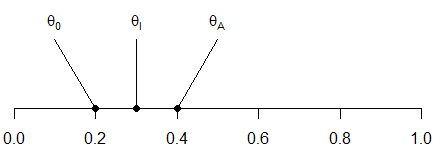
\includegraphics[width=4in]{P:/Git/Bayesian-Sequential-Monitoring/00-paper/FIGURES/line_graph2}
%
%Figure 1: Graph of null response value ($\theta_0$), intermediate response value ($\theta_I)$ and substantial response value $(\theta_A)$.
%\end{center}


%\\
%\int_\Theta \theta p(\theta|\mathbf{D},\pi_{I})d\theta&=\omega\cdot \int_\Theta \theta p(\theta|\mathbf{D},\pi_{S})d\theta+(1-\omega)\cdot\int_\Theta \theta %p(\theta|\mathbf{D},\pi_{E})d\theta
%\begin{align*}
%\pi_{Inference}=\frac{p(\mathbf{D}| \pi_{S}) \pi_{S}+p(\mathbf{D}| \pi_{E}) \pi_{E}}{p(\mathbf{D}| \pi_{S})+p(\mathbf{D}| \pi_{E})}
%\end{align*}
%\begin{align*}
%E(\theta|\mathbf{D},\pi_{Inference})=\omega\times E(\theta|\mathbf{D}, \pi_{S})+(1-\omega)\times E(\theta|\mathbf{D}, \pi_{E})
%\end{align*}
%Need to describe relation to Type I and Type II error.
%\subsubsection{Default parameterization of monitoring priors for common designs}\label{monitoring_prior_specification}
%Define prior distribution as $\pi(\theta|\lambda)$ where $\lambda$ is a vector of hyperparameters.

%Reference prior attempts to express no particular opinion about the treatment's merit. 



%\subsection{Futility Monitoring Using Probability of Success (EVAN -- draft on 6/21)}
%
%\begin{itemize}
% \item Futility monitoring using POS is about stopping early when their is a high likelihood
%       of a study being inconclusive at the end of the study.
% \item Since the final analysis uses the \textit{Inference} prior, POS should be based on the
%       inference prior.
% \item Develop the framework for POS and show how it is a weighted average POS based on the skeptical
%       and enthusiastic priors.
%\end{itemize}


%Stochastic curtailment in frequentist setting.
\section{Examples}

\subsection{Single-Arm Proof-of-Activity Trial with Binary Endpoint}
\subsubsection{Motivating example}
Consider a single-arm proof-of-activity trial with a binary endpoint. The data $\mathbf{D}$ are binomially distributed and the response rate $\theta$ is the parameter of interest, with higher values of $\theta$ being indicative of proof-of-activity. 

An example application is based on the drug iniximab, which is FDA approved for the treatment of several diseases, including ulcerative colitis (UC). The goal of the trial is to test the hypothesis: $H_0:\theta\leq\theta_0=0.40$ versus $H_1:\theta>\theta_0$. From adult data $\theta_1=0.67$. Based on the 54-week follow-up period, we can infer enrollment took place over approximately 33 months (approximately 1 patient per 0.55 months).

\subsubsection{Model formulation \& prior elicitation}
The default skeptical and enthuastic priors will be of the form (\ref{eq:generalized_normal_univariate}) with $\beta=2$ corresponding to truncated normal distributions
\begin{align*}
\pi_S(\theta)&\propto \exp\left\{-\frac{(\theta-\theta_0)}{\alpha_S}^2\right\} I(\theta\in[0,1])\\
\pi_E(\theta)&\propto \exp\left\{-\frac{(\theta-\theta_1)}{\alpha_E}^2\right\} I(\theta\in[0,1])
\end{align*}
with $\alpha_S$ and $\alpha_E$ chosen satisfy (\ref{eq:enth_prior}) and (\ref{eq:skpt_prior}), where $\Theta_1=(\theta_0,1]$, $\Theta_A=[\theta_1,1]$, and $\epsilon=0.025$.

Alternative specifications of the priors will be used to concentrate or flatten the distribution around the modal value, which still satisfy conditions (\ref{eq:enth_prior}) and (\ref{eq:skpt_prior}). In particular, the skeptical prior can be concentrated around the modal value $\theta_0$ by increasing the mass located in the interval $[\theta_0,\frac{\theta_0+\theta_1}{2})$ and the enthuastic prior can be flattened around the modal value of $\theta_1$ by decreasing the mass located in the interval $(\frac{\theta_0+\theta_1}{2},\theta_1]$.

\begin{center}
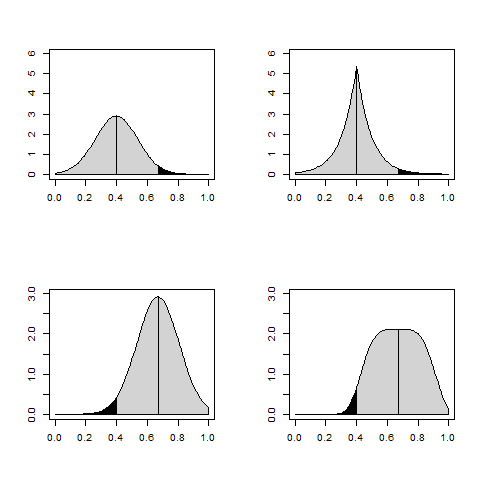
\includegraphics[width=6in]{P:/Git/Bayesian-Sequential-Monitoring/00-paper/FIGURES/figure1.png}

Figure 1: (a) Default skeptical prior ($\beta=2)$ (b) Concentrated skeptical prior\\ (c) Default enthuastic prior ($\beta=2)$ (d) Flattened enthaustic prior
\end{center}

%Beta priors for $\theta$ will be used to provide closed-form expressions of the posterior distributions via Beta-Binomial conjugacy. In particular, let $y_1$ be the number of successes and $y_0$ be the number of failures. If the skeptical prior is $\pi_S(\theta)\sim\mathcal{B}(\alpha_S,\beta_S)$ then the associated posterior is $p(\theta|\mathbf{D},\pi_S)\sim\mathcal{B}(\alpha_S+y_1,\beta_S+y_0)$. Similarly, if the enthuastic prior is $\pi_E(\theta)\sim\mathcal{B}(\alpha_E,\beta_E)$ then the associated posterior is $p(\theta|\mathbf{D},\pi_E)\sim\mathcal{B}(\alpha_E+y_1,\beta_E+y_0)$.

%\begin{center}
%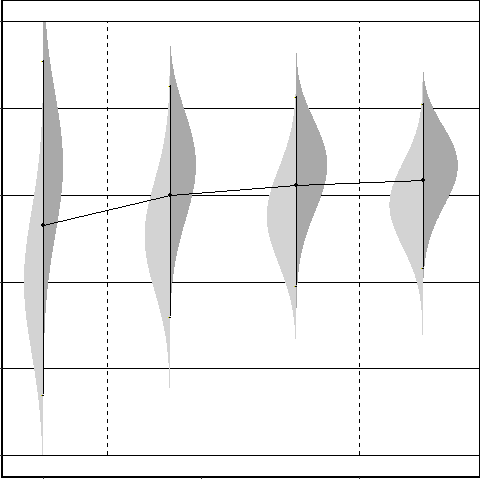
\includegraphics[width=5in]{P:/Git/Bayesian-Sequential-Monitoring/00-paper/FIGURES/violin_efficacy.png}
%\end{center}
%\begin{center}
%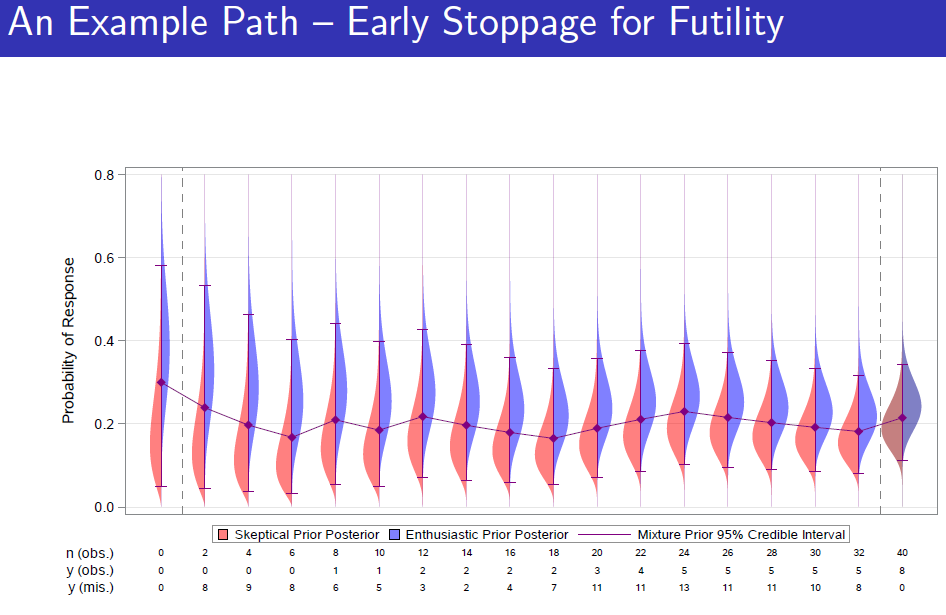
\includegraphics[width=5in]{P:/Git/Bayesian-Sequential-Monitoring/00-paper/FIGURES/violin_futility.png}
%\end{center}

The following analyses are done with the concentrated skeptical prior and the default enthuastic prior.
\subsubsection{Sequential monitoring}
Enrollment will proceed until one of the following three conditions are satisfied:
\begin{align*}
\text{Efficacy criteria (EFF): }&P(\theta>\theta_0|\mathbf{D},\pi_S)\geq 0.975\\
\text{Futility criteria (FUT): }&P\left(\theta\leq\frac{\theta_0+\theta_1}{2} \Big|\mathbf{D},\pi_E\right)\geq 0.975\\
\text{Maximum sample size: }&N=112 \text{ patient outcomes obtained}
\end{align*}
Assume that the outcomes are ascertained after approximately 4 months of follow-up and 2 patients per month on average are enrolled. If enrollment is terminated due to the efficacy or futility criteria being satisfied, those subjects who are still undergoing follow-up will still have their outcomes considered in the final analysis.
\subsubsection{Example paths}
To demonstrate the monitoring procedure, two example trials are considered. 
%As seen in Figure 3(a), at the second interim analysis the efficacy condition $P(\theta>0.20|\mathbf{D},\pi_S)\geq 0.95$ is satisfied and enrollment is terminated. As shown in Figure 3(b), at the fourth interim analysis the futility condition $P(\theta\leq 0.30|\mathbf{D},\pi_E)\geq 0.85$ is satisfied and enrollment is terminated. In both examples there are subjects with missing outcomes, which are those who are still undergoing follow-up. The final analysis incorporates the final sample.
\begin{center}
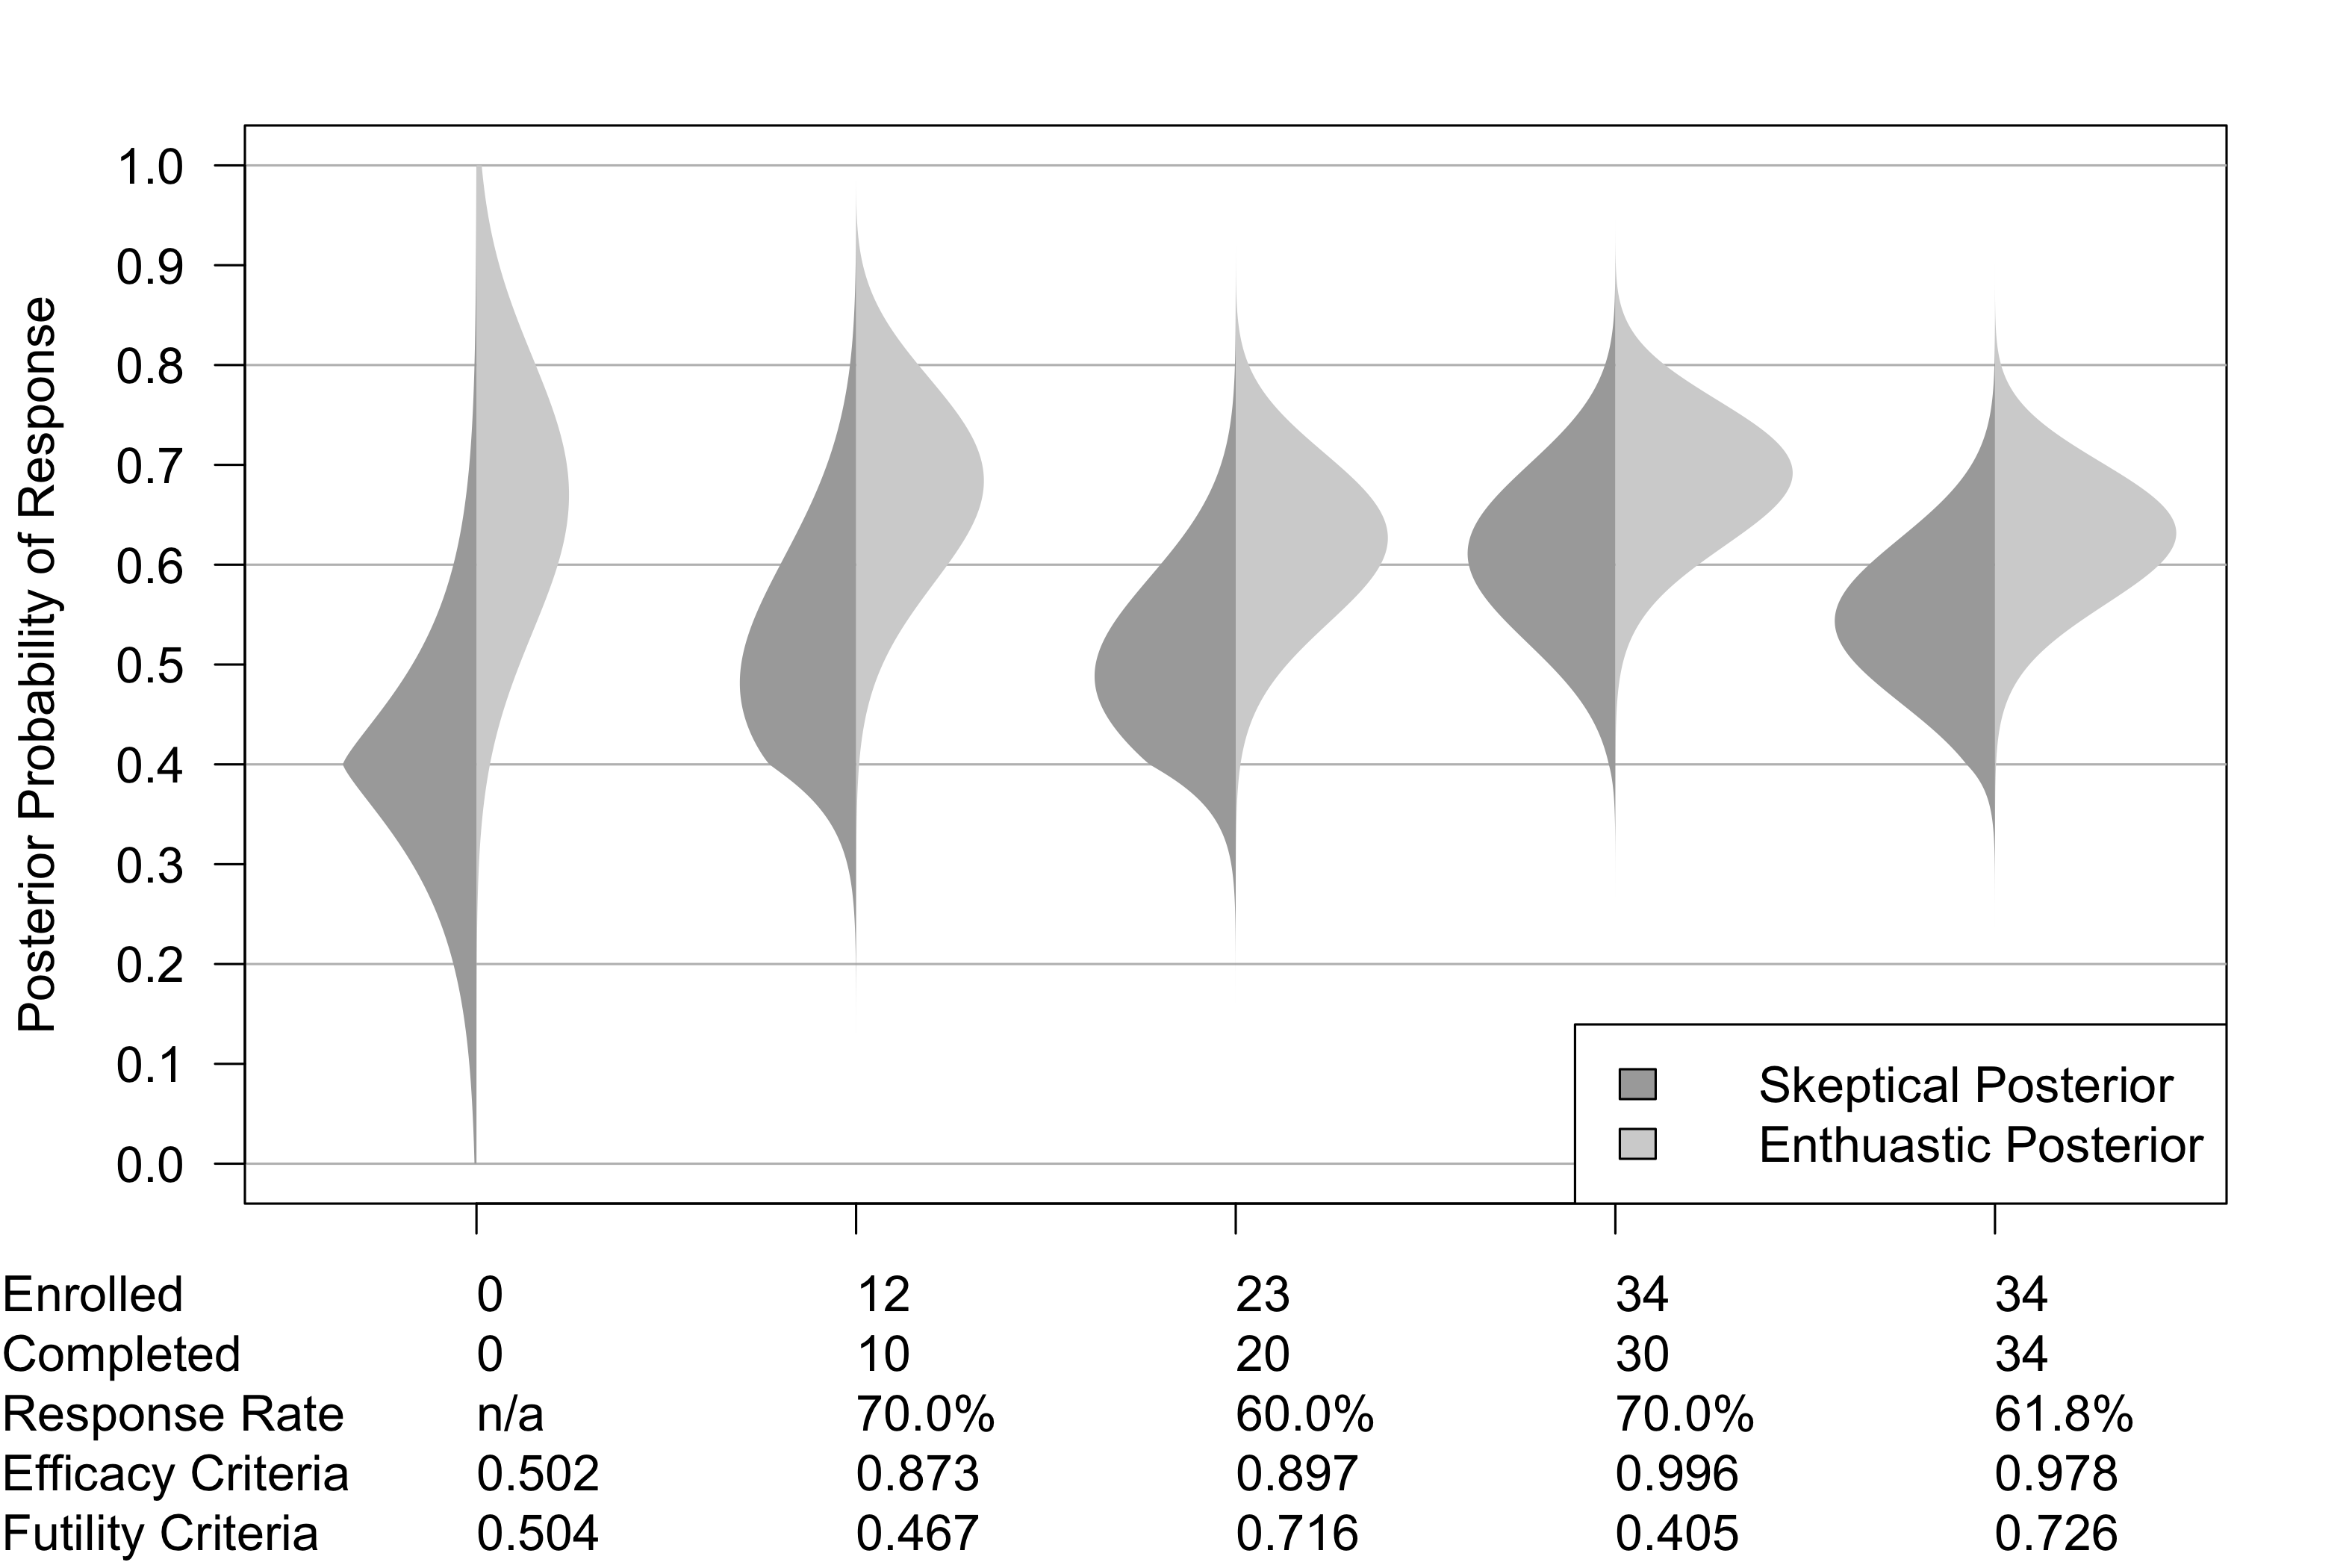
\includegraphics[width=4.5in]{P:/Git/Bayesian-Sequential-Monitoring/00-paper/FIGURES/figure2a.png}
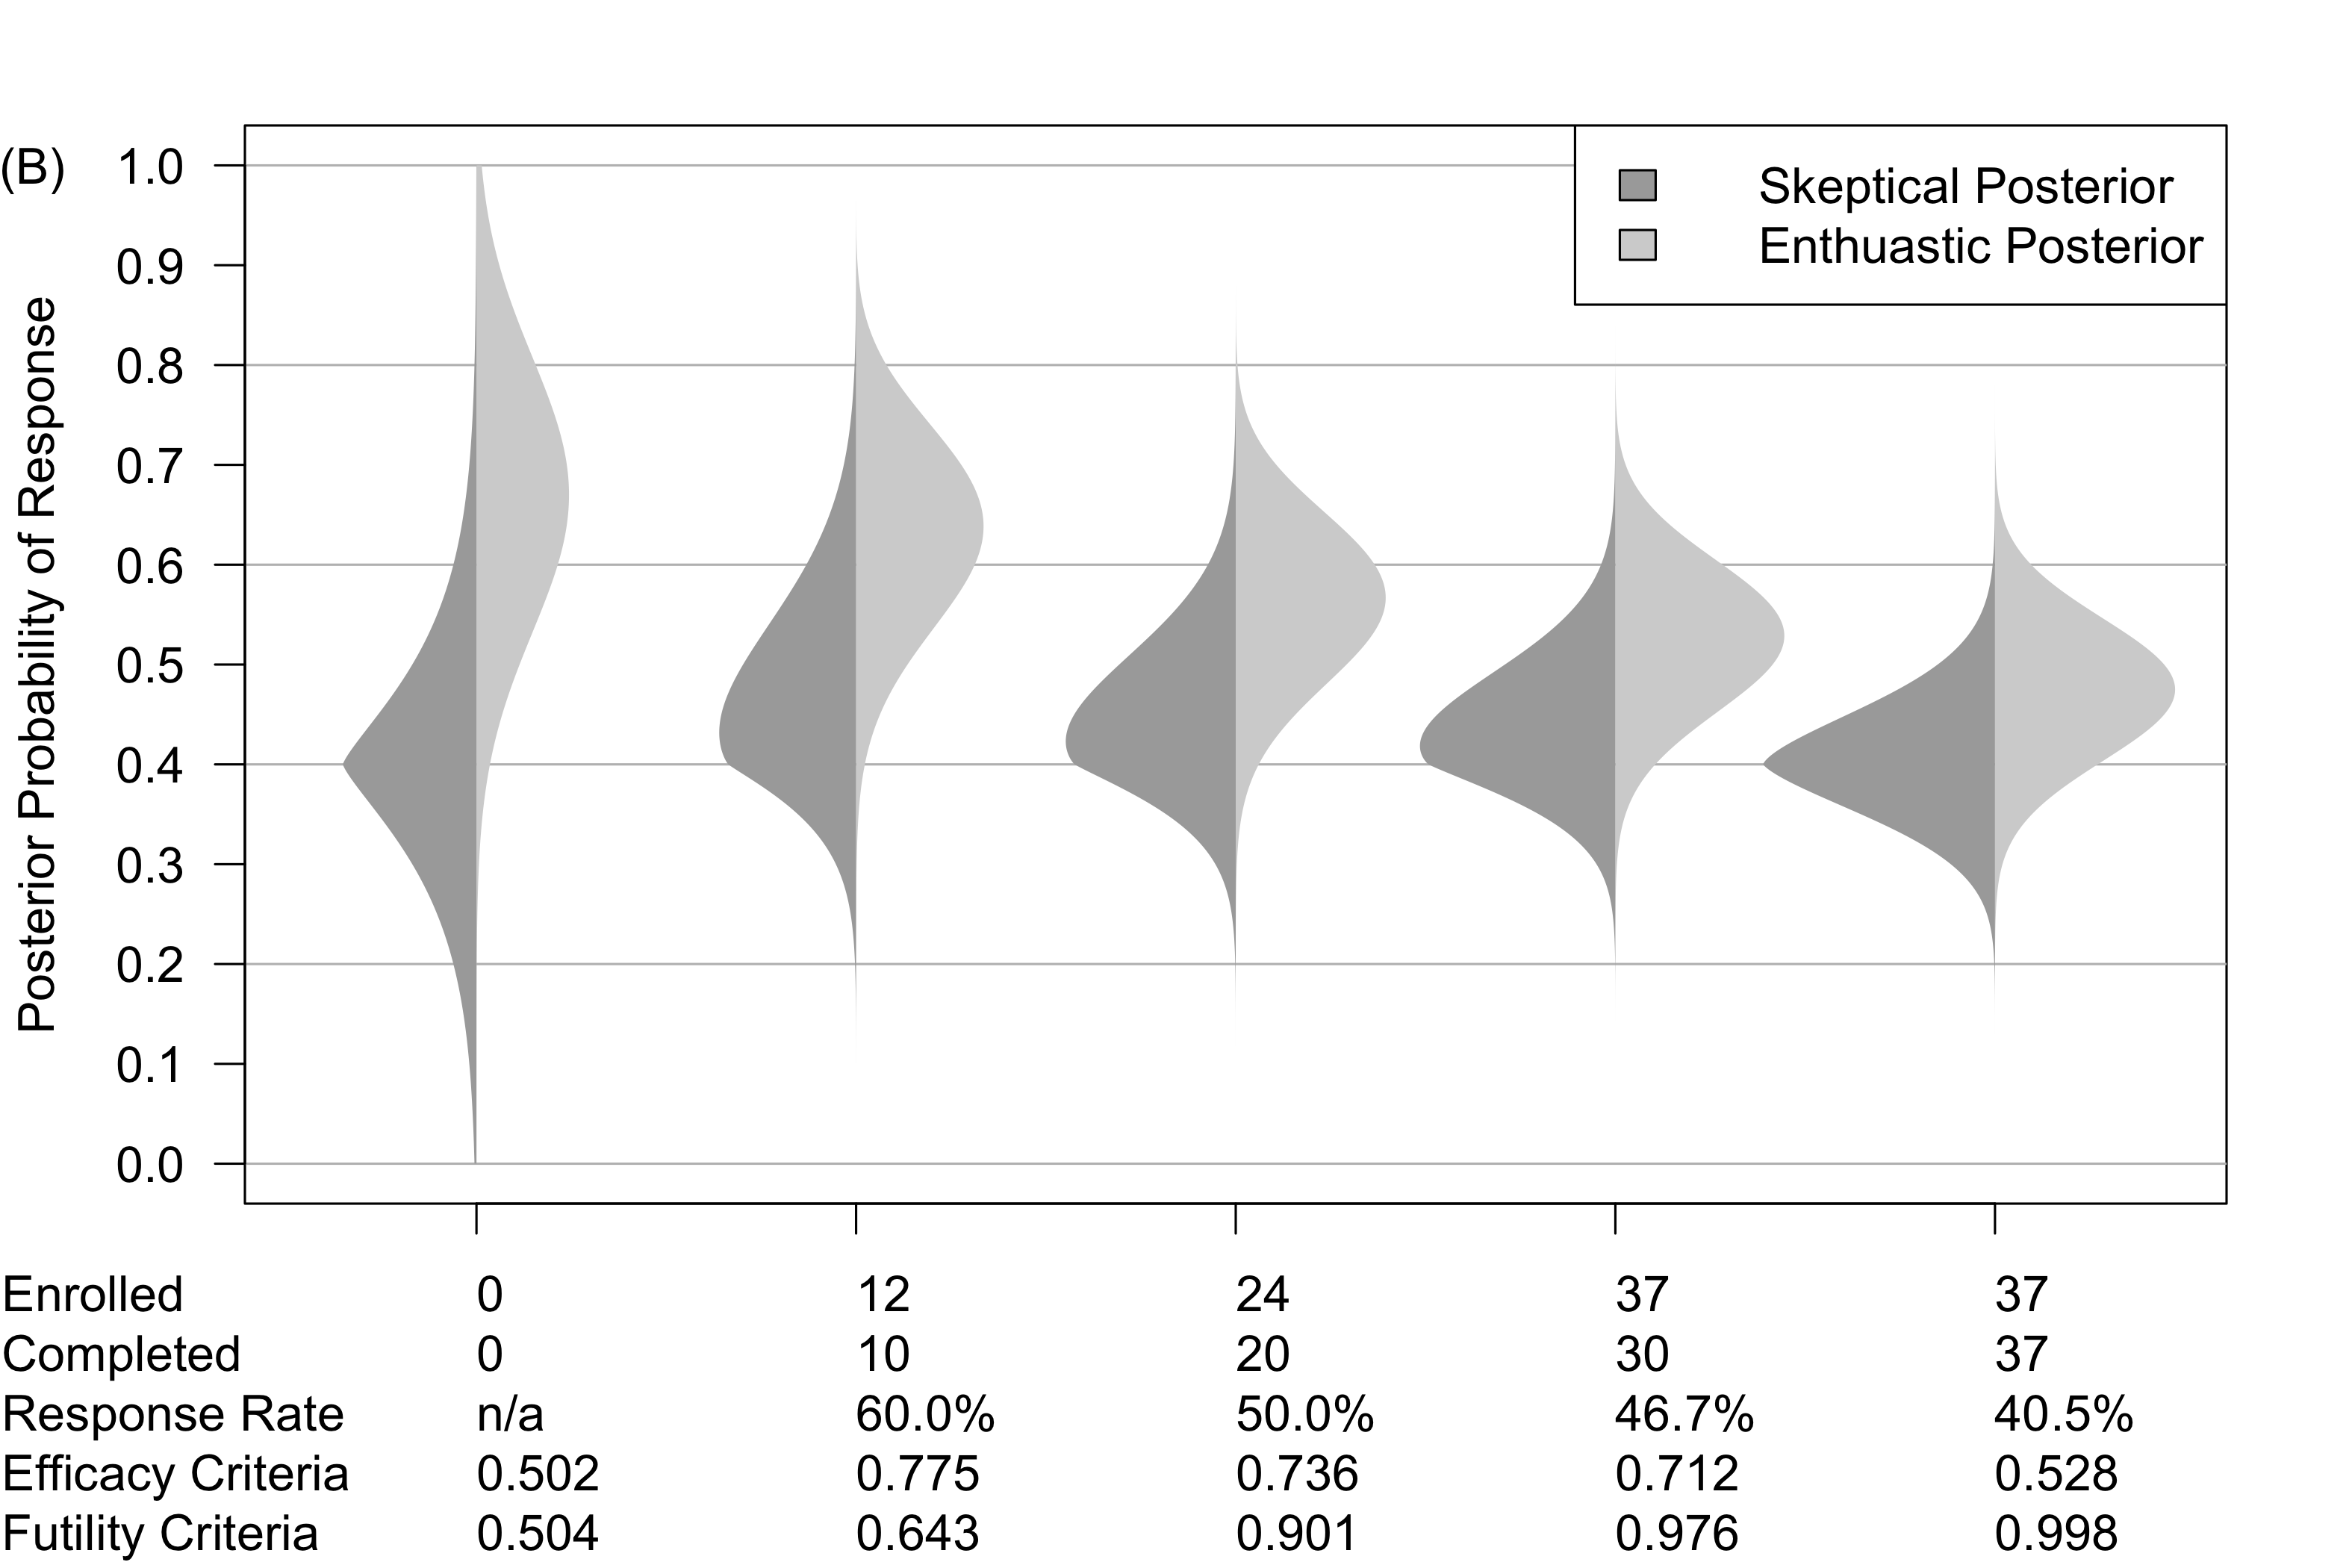
\includegraphics[width=4.5in]{P:/Git/Bayesian-Sequential-Monitoring/00-paper/FIGURES/figure2b.png}
%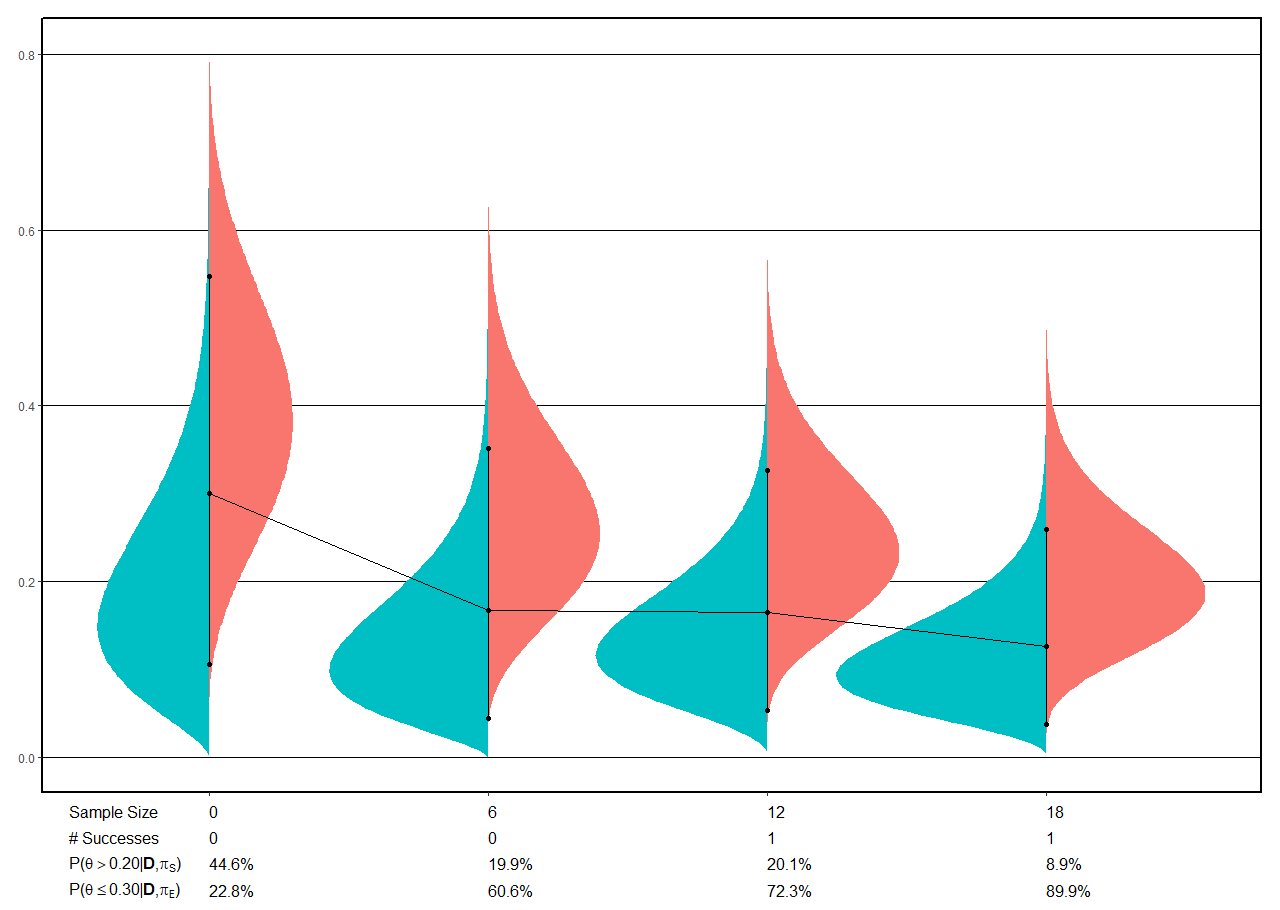
\includegraphics[width=3.5in]{P:/Git/Bayesian-Sequential-Monitoring/00-paper/FIGURES/violin_futility_ekk.png}

Figure 3: (a) Early stopping for efficacy (b) Early stopping for futility
\end{center}
\newpage
\subsubsection{Preposterior Analysis of Operating Characteristics}
An interim analysis will be completed after every 2 subjects complete follow-up.
\begin{center}
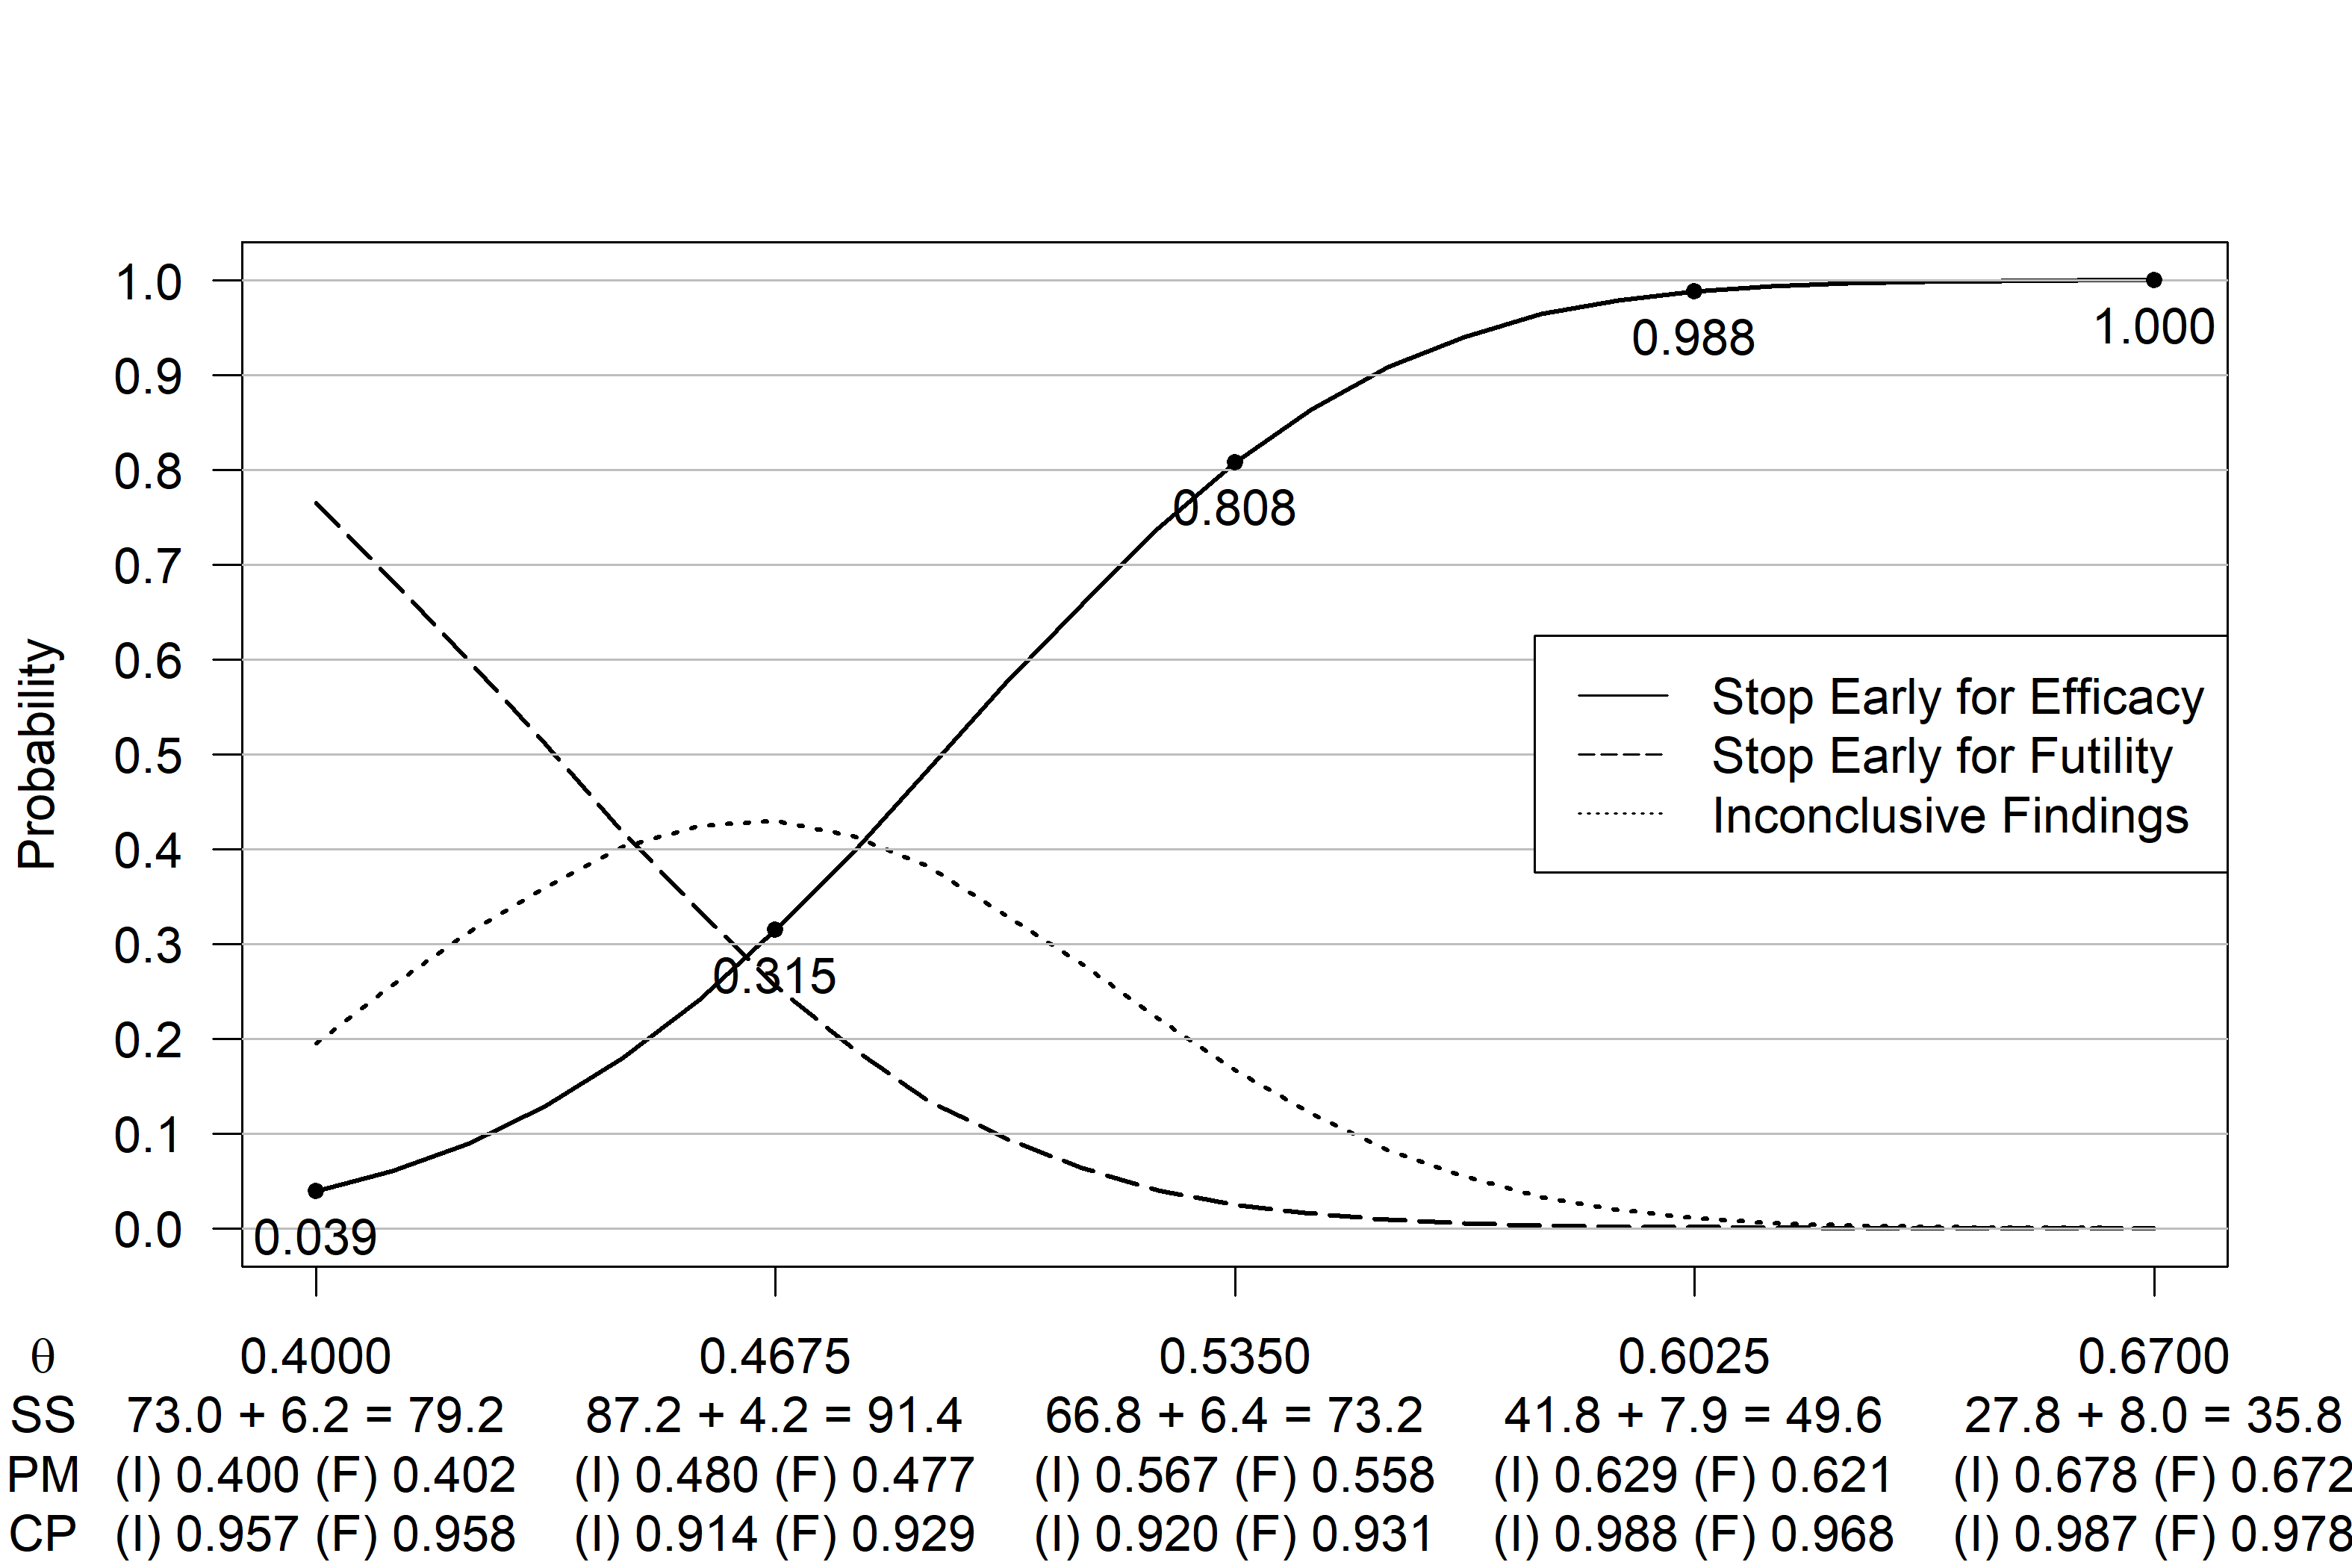
\includegraphics[width=7.5in]{P:/Git/Bayesian-Sequential-Monitoring/00-paper/FIGURES/figure3a.png}
Figure 4a: Sequential design properties of proof-of-activity trial
%\caption{}
\end{center}
Let INC be the probability of reaching the maximum sample size without a conclusive monitoring result, let SS be the average sample size at the definitive interim analysis (I) and at the end of follow-up (F), let CP be the coverage probability using the mixture prior, and let PM be the posterior mean an inference prior which is a 50/50 mixture of the skeptical and enthuastic priors.
\subsubsection{Agreement between interim and final result}
\begin{center}
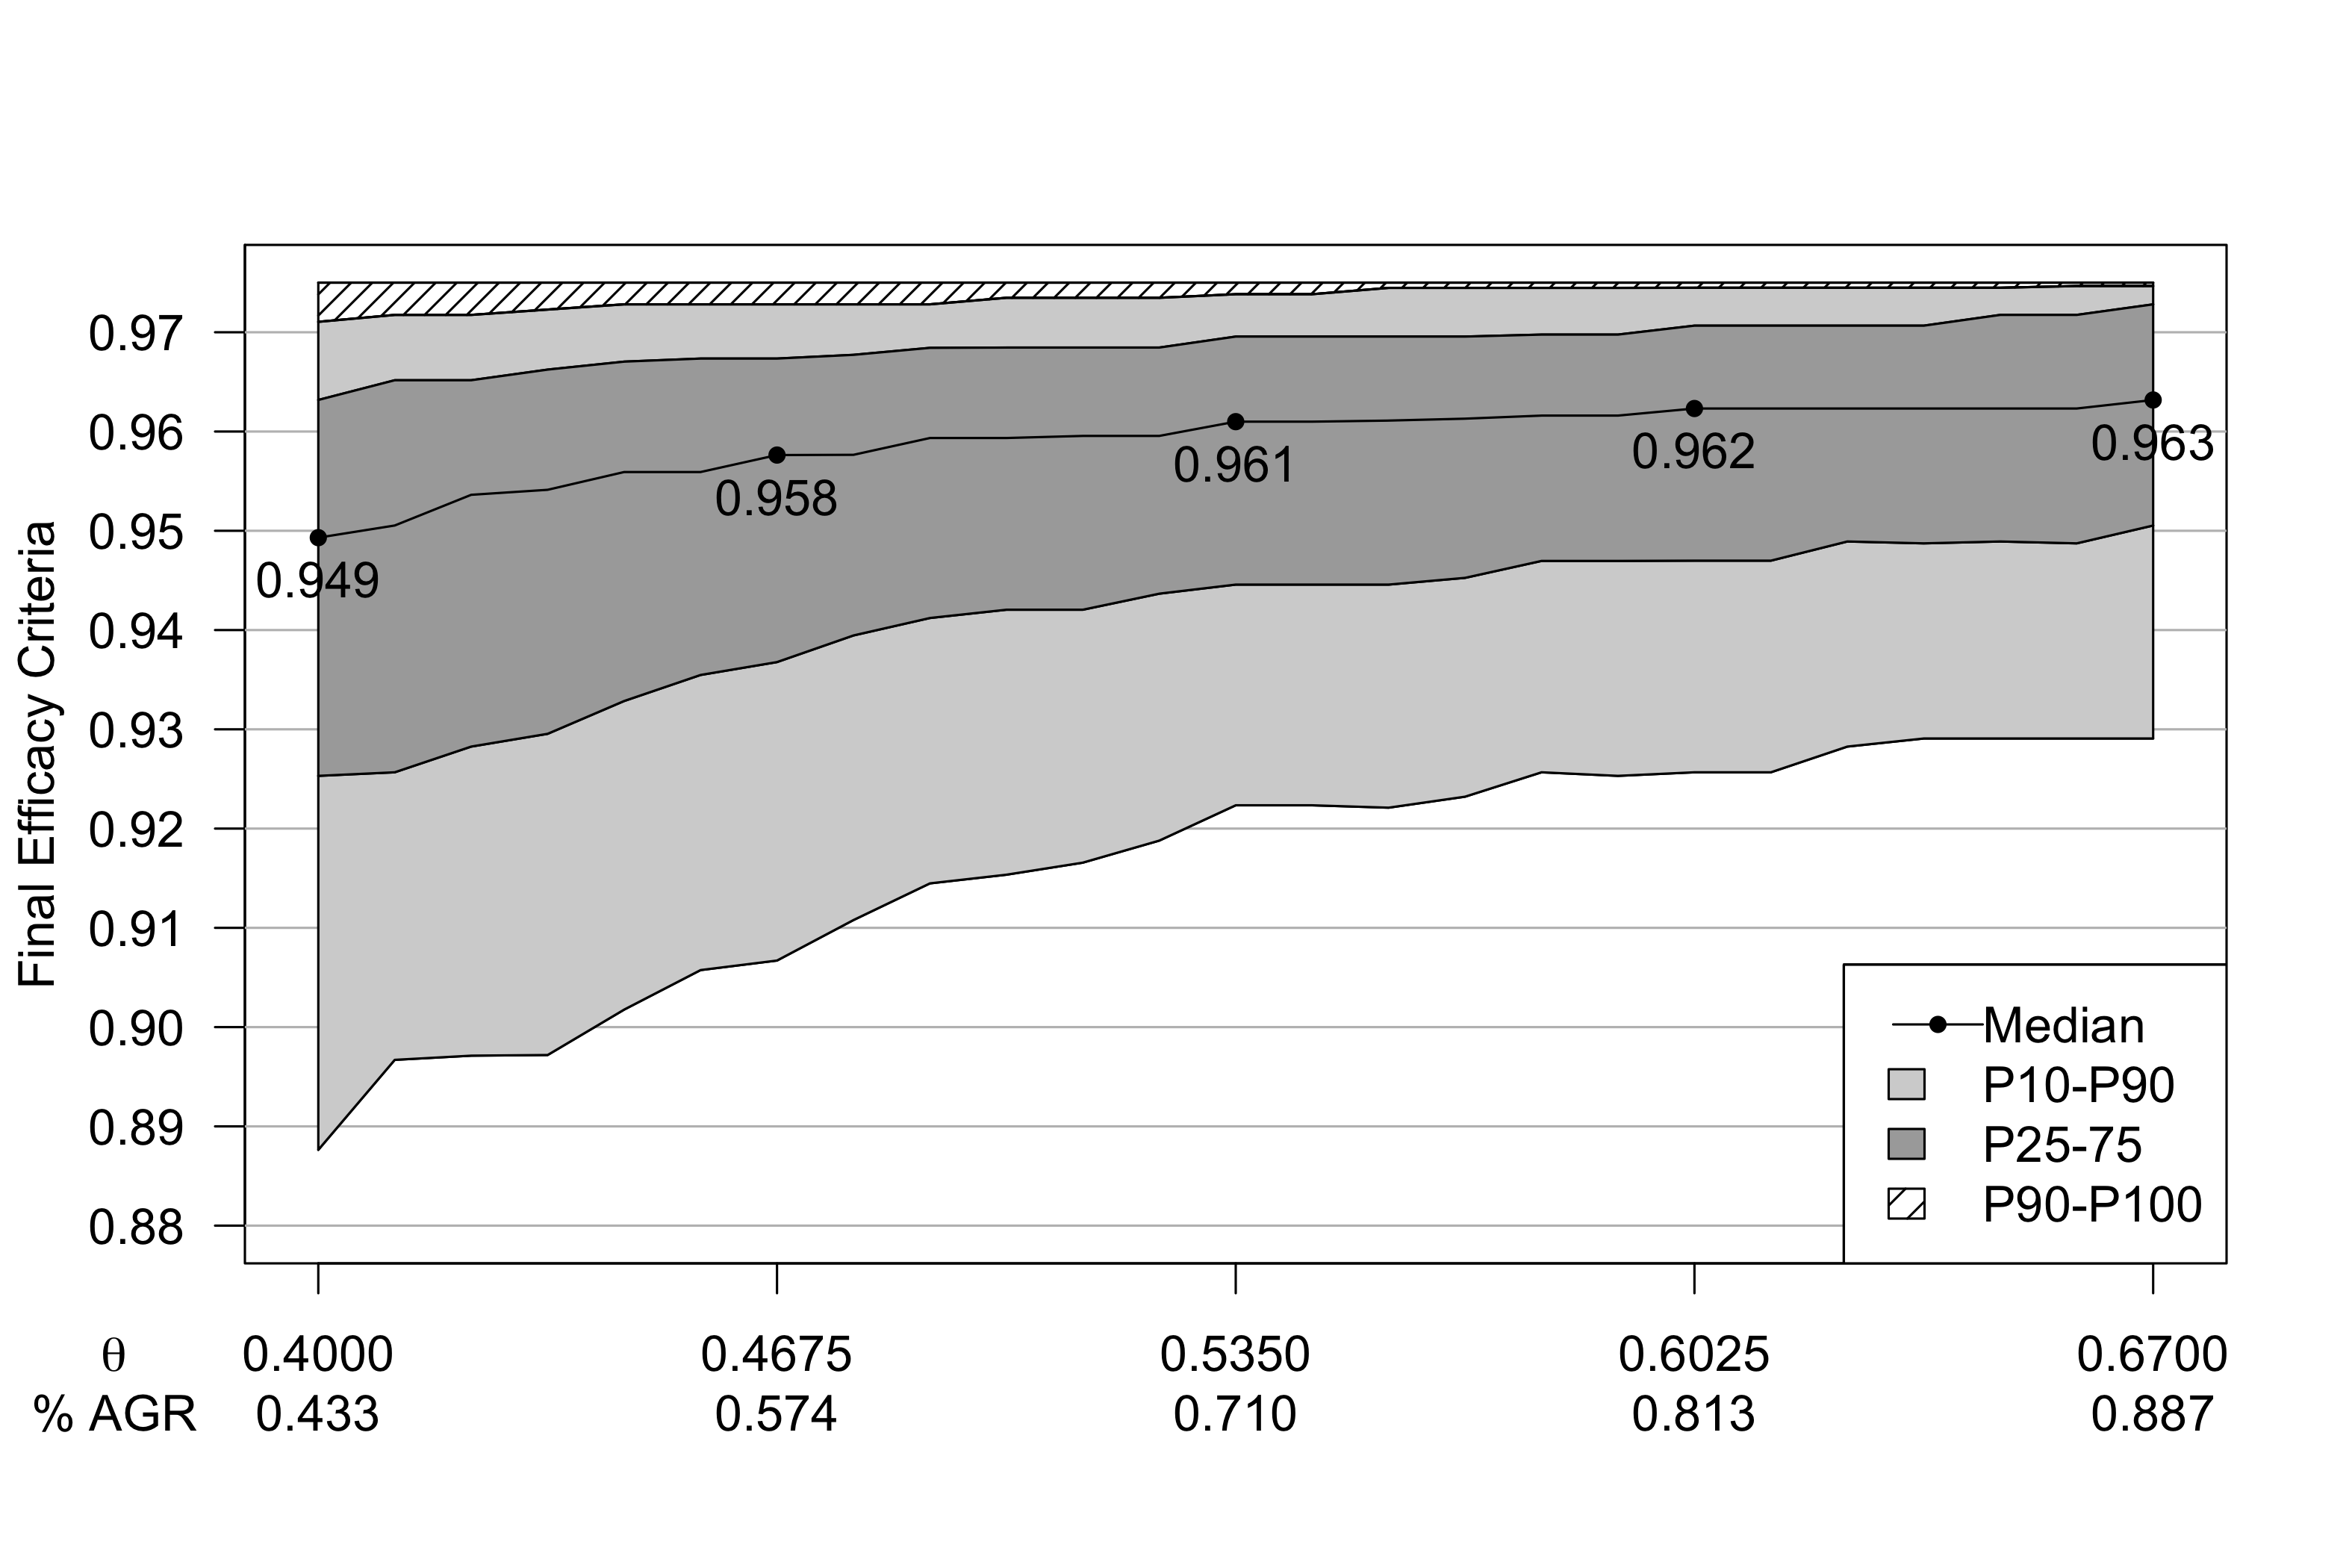
\includegraphics[width=7.5in]{P:/Git/Bayesian-Sequential-Monitoring/00-paper/FIGURES/figure3b.png}
Figure 4b: Percent agreement between interim and final result is listed in AGR. The lower dot is the 10th percentile, middle dot is 25th percentile, upper dot is 50th percentile/median
%\caption{}
\end{center}
%\begin{center}
%Table 1: Distribution of final posterior probability given interim stoppage (interim $P(\theta>0.20|\mathbf{D},\pi_S)\geq 0.95$) and evidence decrease.
%\begin{tabular}{l|ccccccc}
%&0.15&0.20&0.25&0.30&0.35&0.40&0.45\\
%\hline
%Final $P(\theta>0.20|\mathbf{D},\pi_S)\geq 0.95$ &0.293&0.510&0.645&0.753&0.832&0.894&0.932 \\ 
%Final $P(\theta>0.20|\mathbf{D},\pi_S)< 0.95$&0.707&0.490&0.355&0.247&0.168&0.106&0.068\\  
%\hspace{0.5in}Conditional Median&0.91&0.92&0.92&0.93&0.93&0.93&0.93\\  
%\hspace{0.5in}Conditional 25th percentile&0.87&0.89&0.90&0.91&0.91&0.91&0.91\\  
%\hspace{0.5in}Conditional 10th percentile&0.83&0.86&0.87&0.88&0.88&0.88&0.88\\  
%\hspace{0.5in}Conditional 1st percentile&0.67&0.78&0.81&0.81&0.82&0.82&0.82
%\end{tabular}
%\end{center}

%For example, at a true response rate of $\theta=0.40$, there is probability $0.894$ that the threshold for a significant result is maintained after the additional subjects complete follow-up. Conversely, with probability $0.106$ the evidence decreases, and in this case the median posterior probability is $0.93$, and a posterior probability lower than $0.88$ occurs with probability $0.1$. Thus there is a slight attenudation with respect to the dichotomous threshold, but little change in the posterior probability overall.

%\begin{figure}
%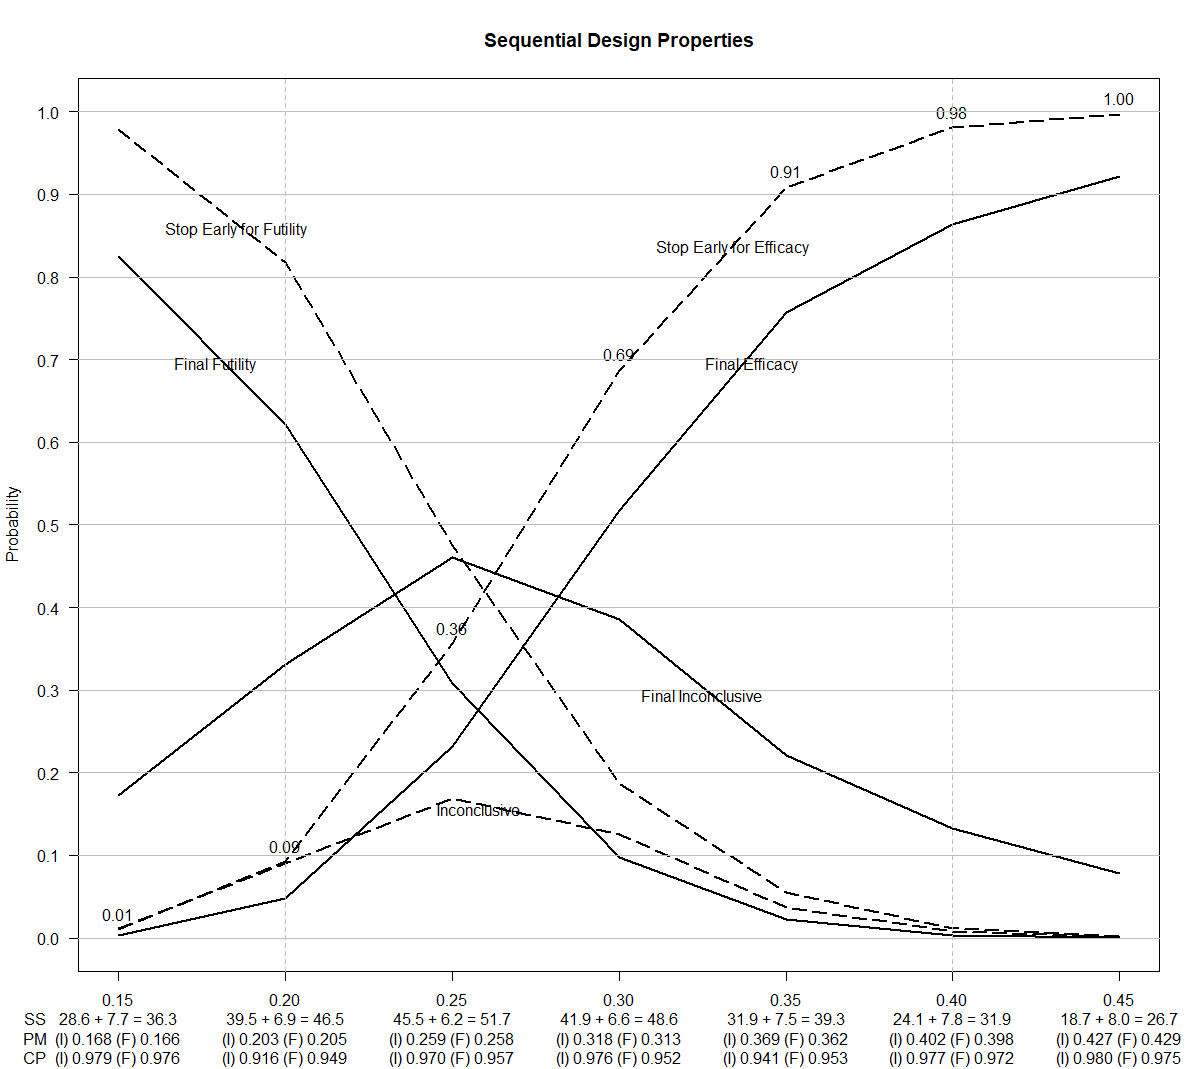
\includegraphics[width=6in]{P:/Git/Bayesian-Sequential-Monitoring/00-paper/FIGURES/sequential_design_properties_2}
%\caption{Shows agreement between sequential and final determinations as they relate to the strict cut-offs}
%\end{figure}

%\subsubsection*{Vemurafenib Trial }
%``In this study, a response rate of 15\% at week
%8 was considered to be low, a response rate of
%45\% was considered to be high, and a response
%rate of 35\% was considered to be low but still
%desirable and indicative of efficacy. Assuming
%response rates as specified in the hypothesis testing, a power of 80\% for a high response rate and
%70\% for the low but still desirable response rate,
%and a two-sided alpha level of 0.1, we calculated
%that the number of patients required in each
%cohort would be 7, 13, or 19, depending on the
%results obtained."
\subsubsection{Type 1 error rate by the frequency of data monitoring}
As expected, the probability of stopping enrollment due to a promising interim trial result and the Type 1 error rate at the final analysis increase with the frequency of interim monitoring, however, the increase is very slight at the final analysis. Regardless of frequency of monitoring there are good Type 1 error rates. 

%Even at the extreme case where an interim analysis is conducted after every outcome, the probability of stopping at the interim due to a promising result when the true response is at the null level is only $0.108$ (about double the nominal rate), and even in this situation the Type 1 error rate once follow-up is complete does not exceed $0.05$. Thus Bayesian sequential monitoring has good frequentist properties even with frequent interim analyses.
%\begin{itemize}
%\item The two sides of the discussion: first is what happens during the trial regarding sequential monitoring, such as \% of time stopping early vs. trial done to completion and expected sample size. Second is the final determination of efficacy or futility and how that relates to Type 1 Error and power. 
%\item  Remember the best case for sequential monitoring is slow enrollment relative to outcome ascertainment. Slow enrollment means there is a benefit to ending trial early and reach a conclusion faster. Outcome ascertainment needs to be somewhat fast to ensure a good \# of outcomes are generated.
%\end{itemize}
%\begin{itemize}
%\item Want to highlight that the ultimate inference will have no Type 1 error inflation. At this point the ultimate inference for efficacy is still made with skeptical prior.
%\item Label lines nicely.
%\item ``Only bad thing to do is to stop learning"
%\item Enrollment rate and \% of ongoing data as operating characteristics are interesting ideas, but focus on the plots already created.
%\item Mat: Scaling on \# of subjects in each interim analysis rather than \# of interim analyses (e.g. flip X axis). Make labels go vertical or diagonal.
%\end{itemize}
\begin{center}
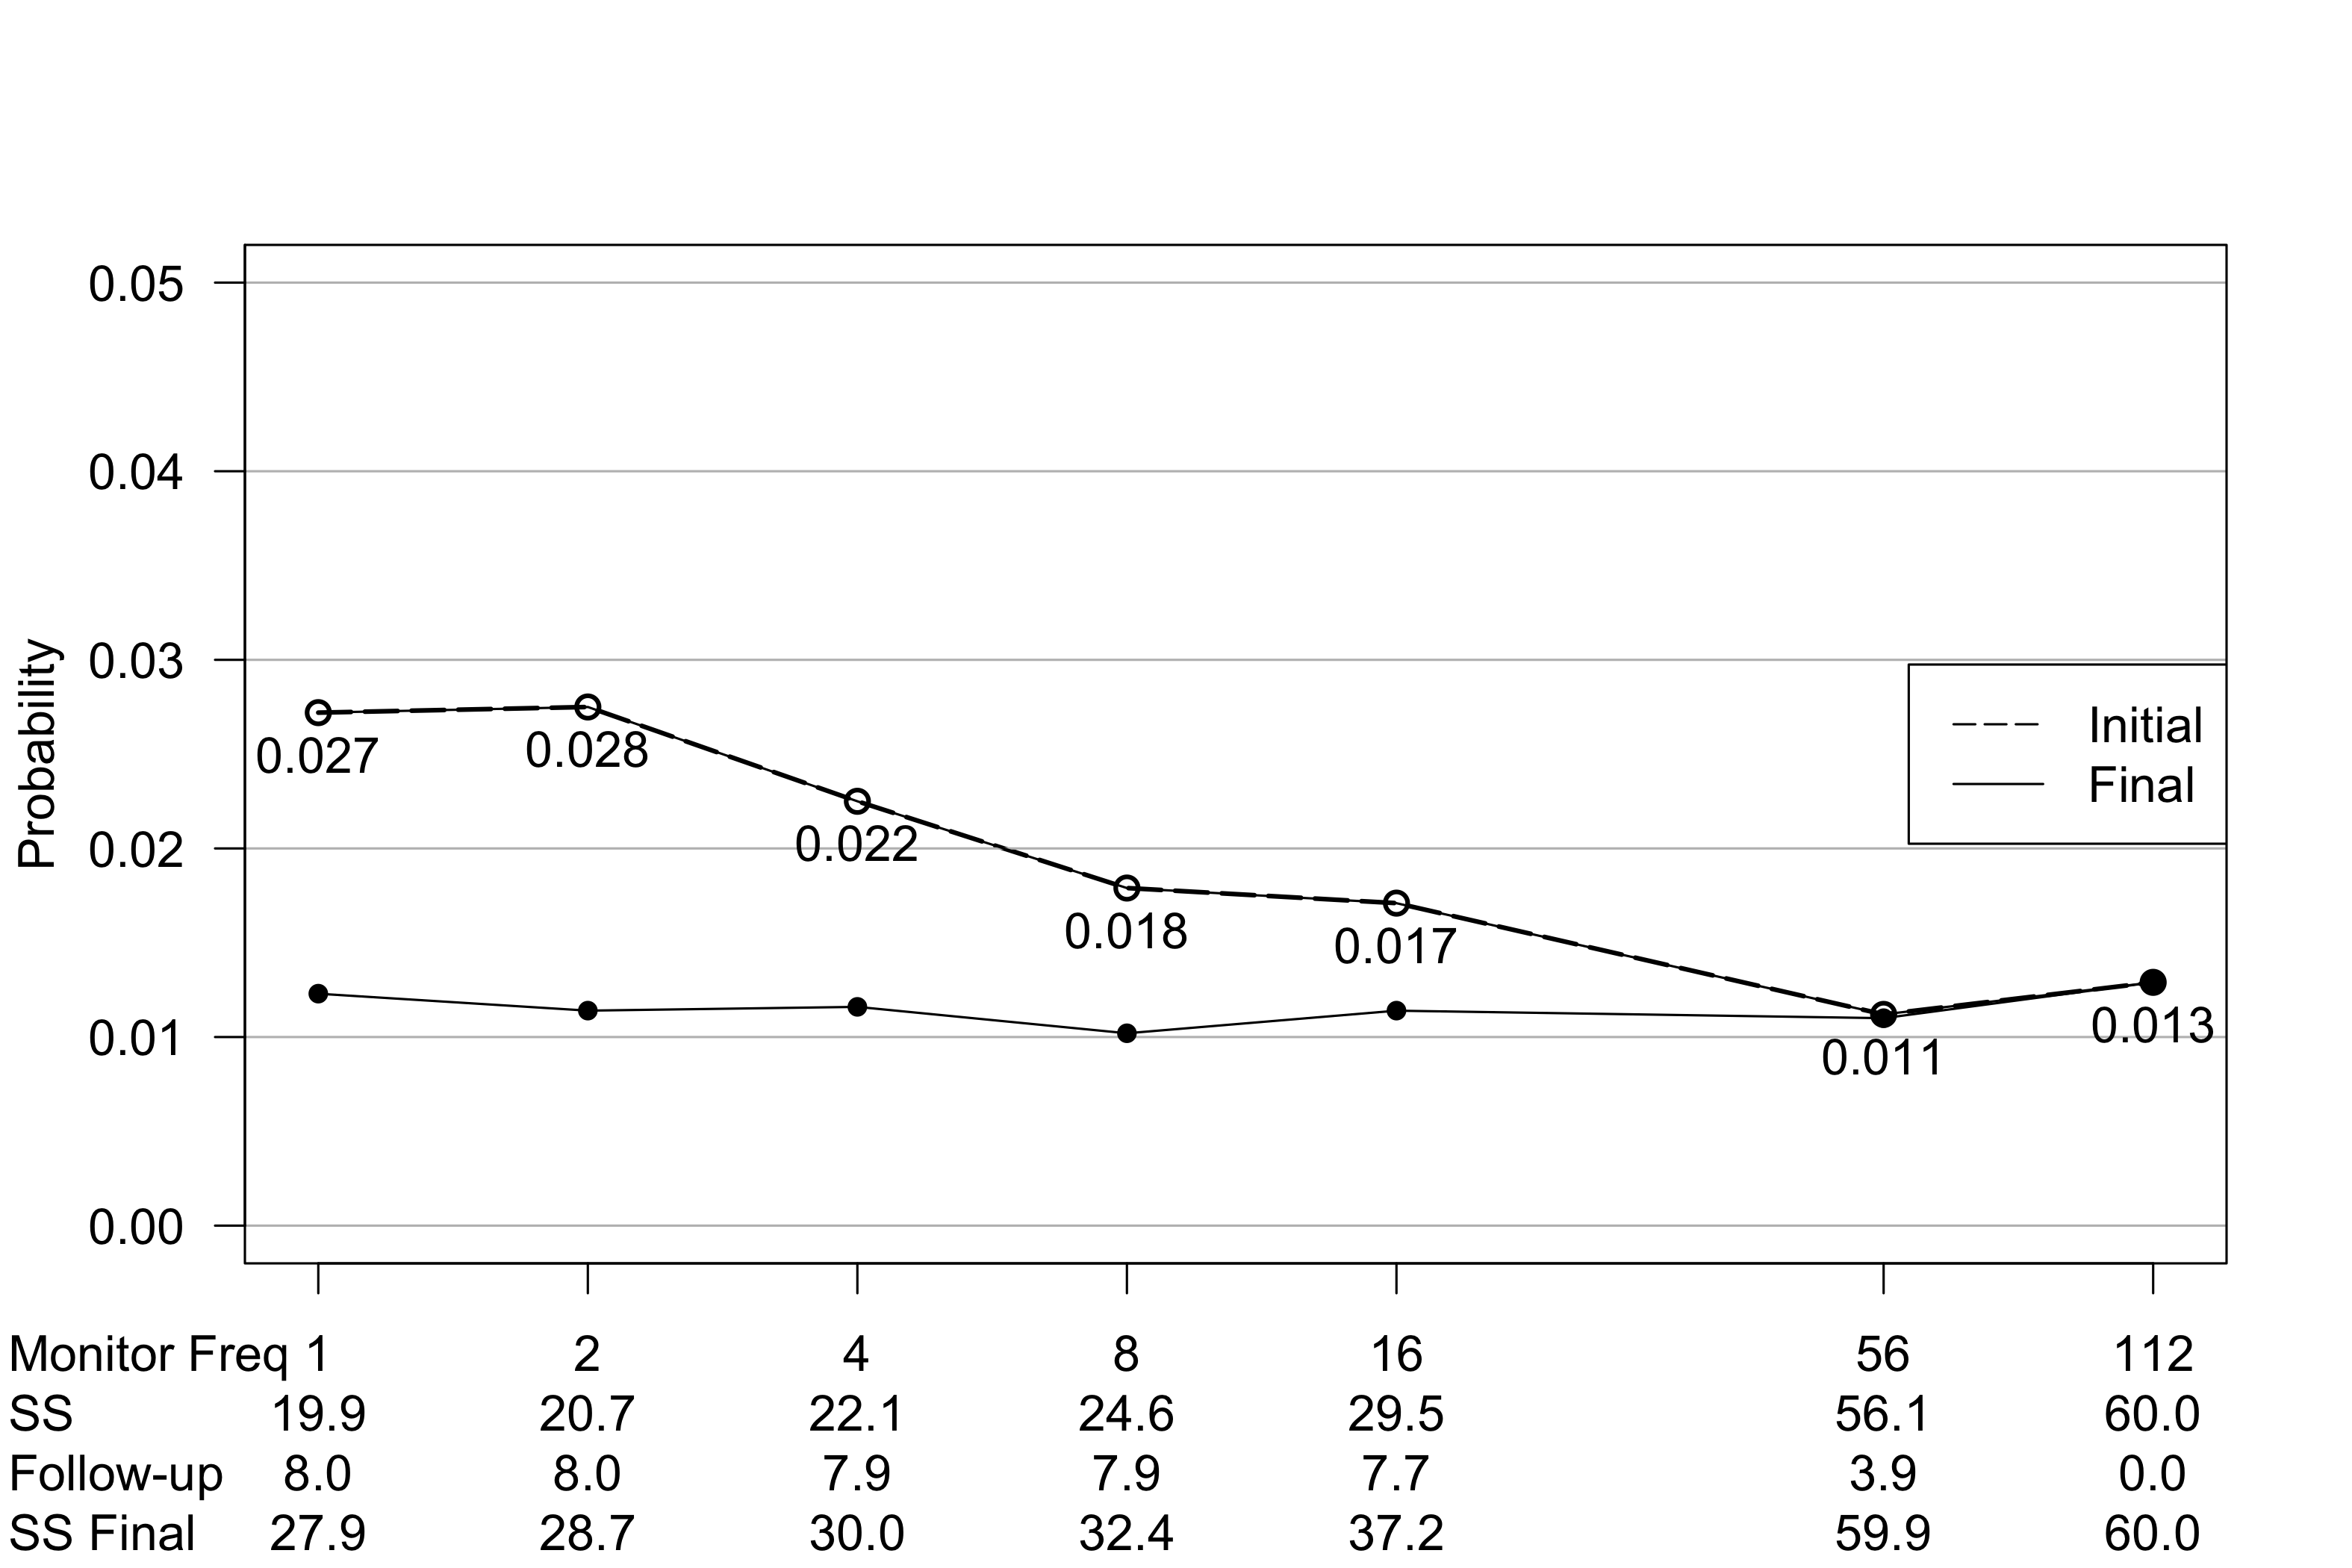
\includegraphics[width=5in]{P:/Git/Bayesian-Sequential-Monitoring/00-paper/FIGURES/figure4.png}

Figure 4: Type 1 error rate depending on frequency of sequential monitoring
\end{center}
Monitoring Freq is 1 for fully sequential design and 112 when the only analysis is with all completed outcomes.
\subsection{Parallel Two-Group Design with Binary Endpoint}
\subsubsection{Motivating example}
The Pediatric Lupus Trial of Belimumab Plus Background Standard Therapy (PLUTO) trial, was a multi-center study to evaluate the safety, pharmacokinetics, and efficacy of belimumab intravenous (IV) in pediatric patients 5 to 17 years of age with active systemic lupus erythematosus. 

The goal was to test for superiority of belimumab to placebo. Based on adult studies, a response rate of $0.51$ was expected for belimumab and based on previous research a response rate of $0.39$ was expected for placebo.

The study design included enrollment of 100 subjects, the first 24 subjects randomized in a 5:1 ratio (belimumab:placebo) and the remaining 76 subjects would be randomized in a 1:1 allocation ratio. Therefore, 58 subjects would be randomized to belimumab and 42 to placebo. The sample size was based on feasibility constraints rather than a power calculation.

The binary response endpoint was evaulated at 52 weeks post enrollment. The study start date was September 7, 2012, and the primary completion date was January 24, 2018. Since the follow-up period is 52 weeks the last enrollment is estimated to be a year prior to the primary completition date yielding an average enrollment rate of one enrollment per $17.2$ days.
\subsubsection{Model formulation}
Let $\theta_0$ represent the response rate the control group and $\theta_1$ represent the response probability for the investigational product (IP) group. 
Consider the hypothesis testing of IP superiority to control
\begin{align*}
H_0:\theta_1-\theta_0\leq 0\text{ vs. }H_1: \theta_1-\theta_0>0.
\end{align*}

The priors will be chosen based on the joint specification in (\ref{eq:generalized_normal_joint}). First, a prior on the response probability for the placebo group is given in the form of (\ref{eq:generalized_normal_PC}). This prior is chosen to be flat in the region $0.39\pm 0.10$.

		\begin{center}
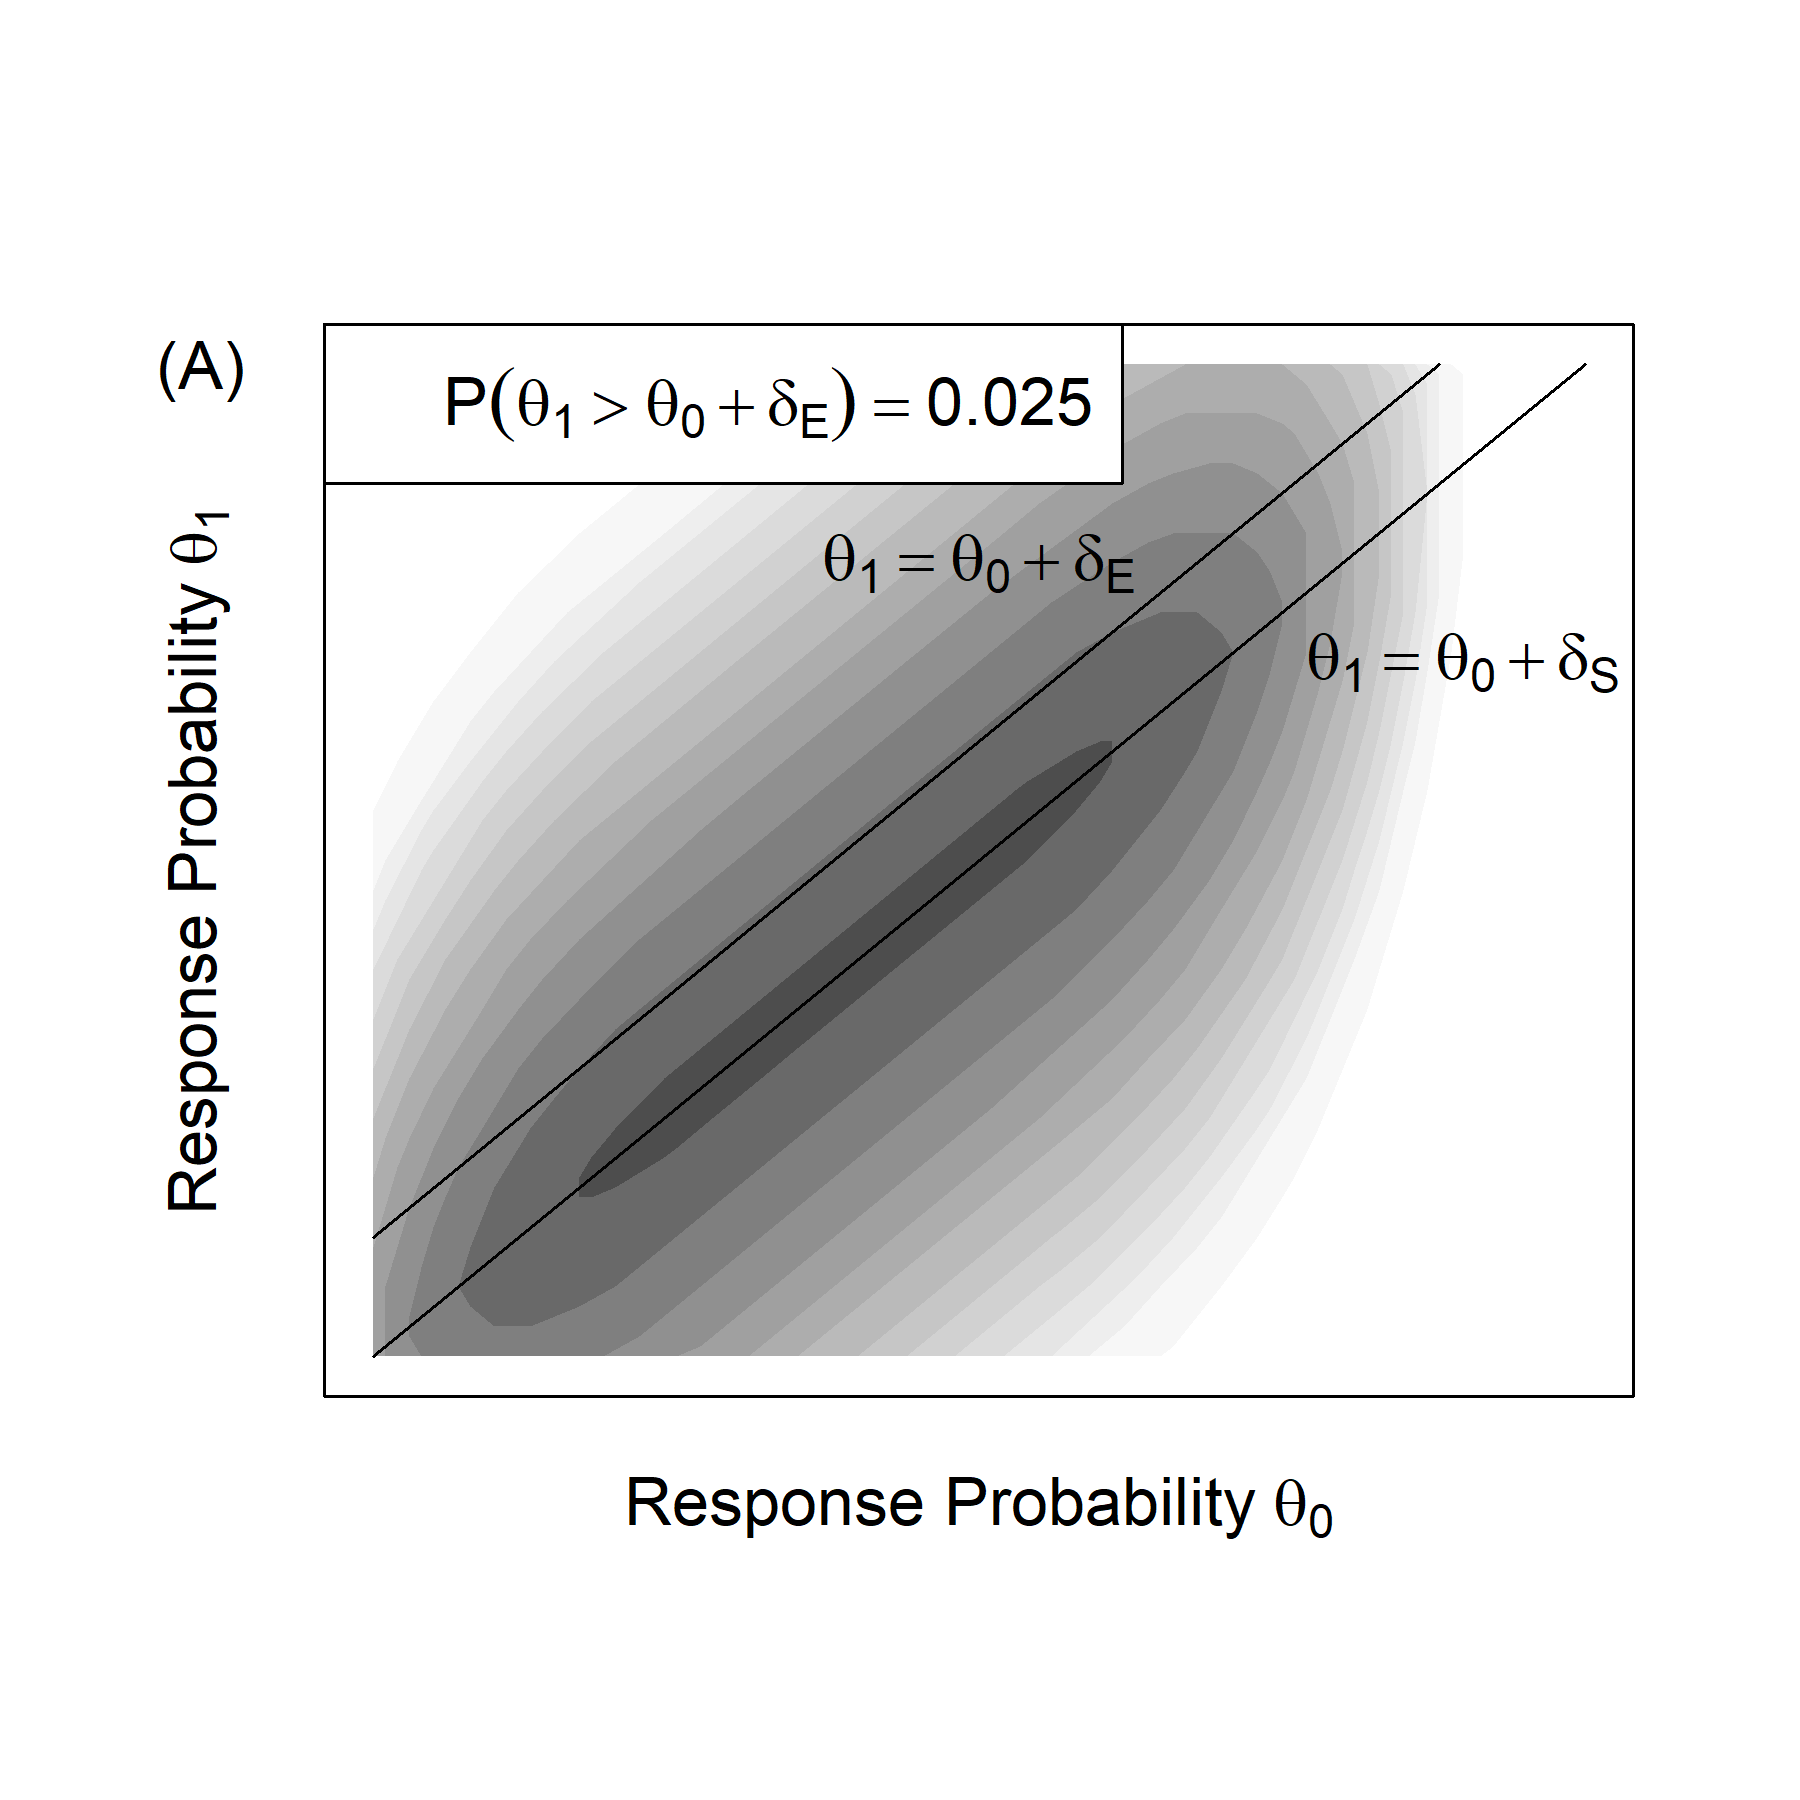
\includegraphics[scale=0.50]{./FIGURES/figure5a.png}
\text{Figure 5a: Prior on placebo response probability in the form of (\ref{eq:generalized_normal_PC}) $(\mu_0=0.39, \alpha_0=0.26, \beta_0=5.3)$}
    \end{center}	




To complete the joint specification of (\ref{eq:generalized_normal_joint}), skeptical and enthuastic priors of the form (\ref{eq:generalized_normal_IP}) will be parameterized as to satisfy (\ref{eq:enth_prior}) and (\ref{eq:skpt_prior}). The skeptic believes there is no difference in response rates by treatment group, and the enthusiastic person believes the IP group will have a response rate probability that is 0.12 higher than the placebo group. 

%This corresponds to $\delta_S=0$ and $\delta_E=0.12$. The skeptical and enthuastic priors are defined as
%\begin{align*}
%\pi_S(\theta_0,\theta_1)=&\exp\left\{-\frac{1}{2}\left(\frac{\theta_0-\mu}{\sigma_S}\right)^{2}\right\}\times \exp\left\{-\frac{1}{2}\left(\frac{(\theta_1-\theta_0)-\delta_S}{\sigma_{S1}}\right)^{2}\right\}\times I((\theta_0,\theta_1)\in [0,1]\times[0,1]) /c_S,\\
%\pi_E(\theta_0,\theta_1)=&\exp\left\{-\frac{1}{2}\left(\frac{\theta_0-\mu}{\sigma_E}\right)^{2}\right\}\times \exp\left\{-\frac{1}{2}\left(\frac{(\theta_1-\theta_0)-\delta_E}{\sigma_{E1}}\right)^{2}\right\}\times I((\theta_0,\theta_1)\in [0,1]\times[0,1]) /c_E
%\end{align*}
%
%where $c_S$ and $c_E$ are normalizing constants. The values of $\sigma_S$ and $\sigma_{S1}$ are chosen such that $P(\theta_1-\theta_0>0.1|\pi_S)=0.05$. Similarly, $\sigma_E$ and $\sigma_{E1}$ are chosen such that $P(\theta_1-\theta_0\leq0|\pi_E)=0.05$.

		\begin{center}
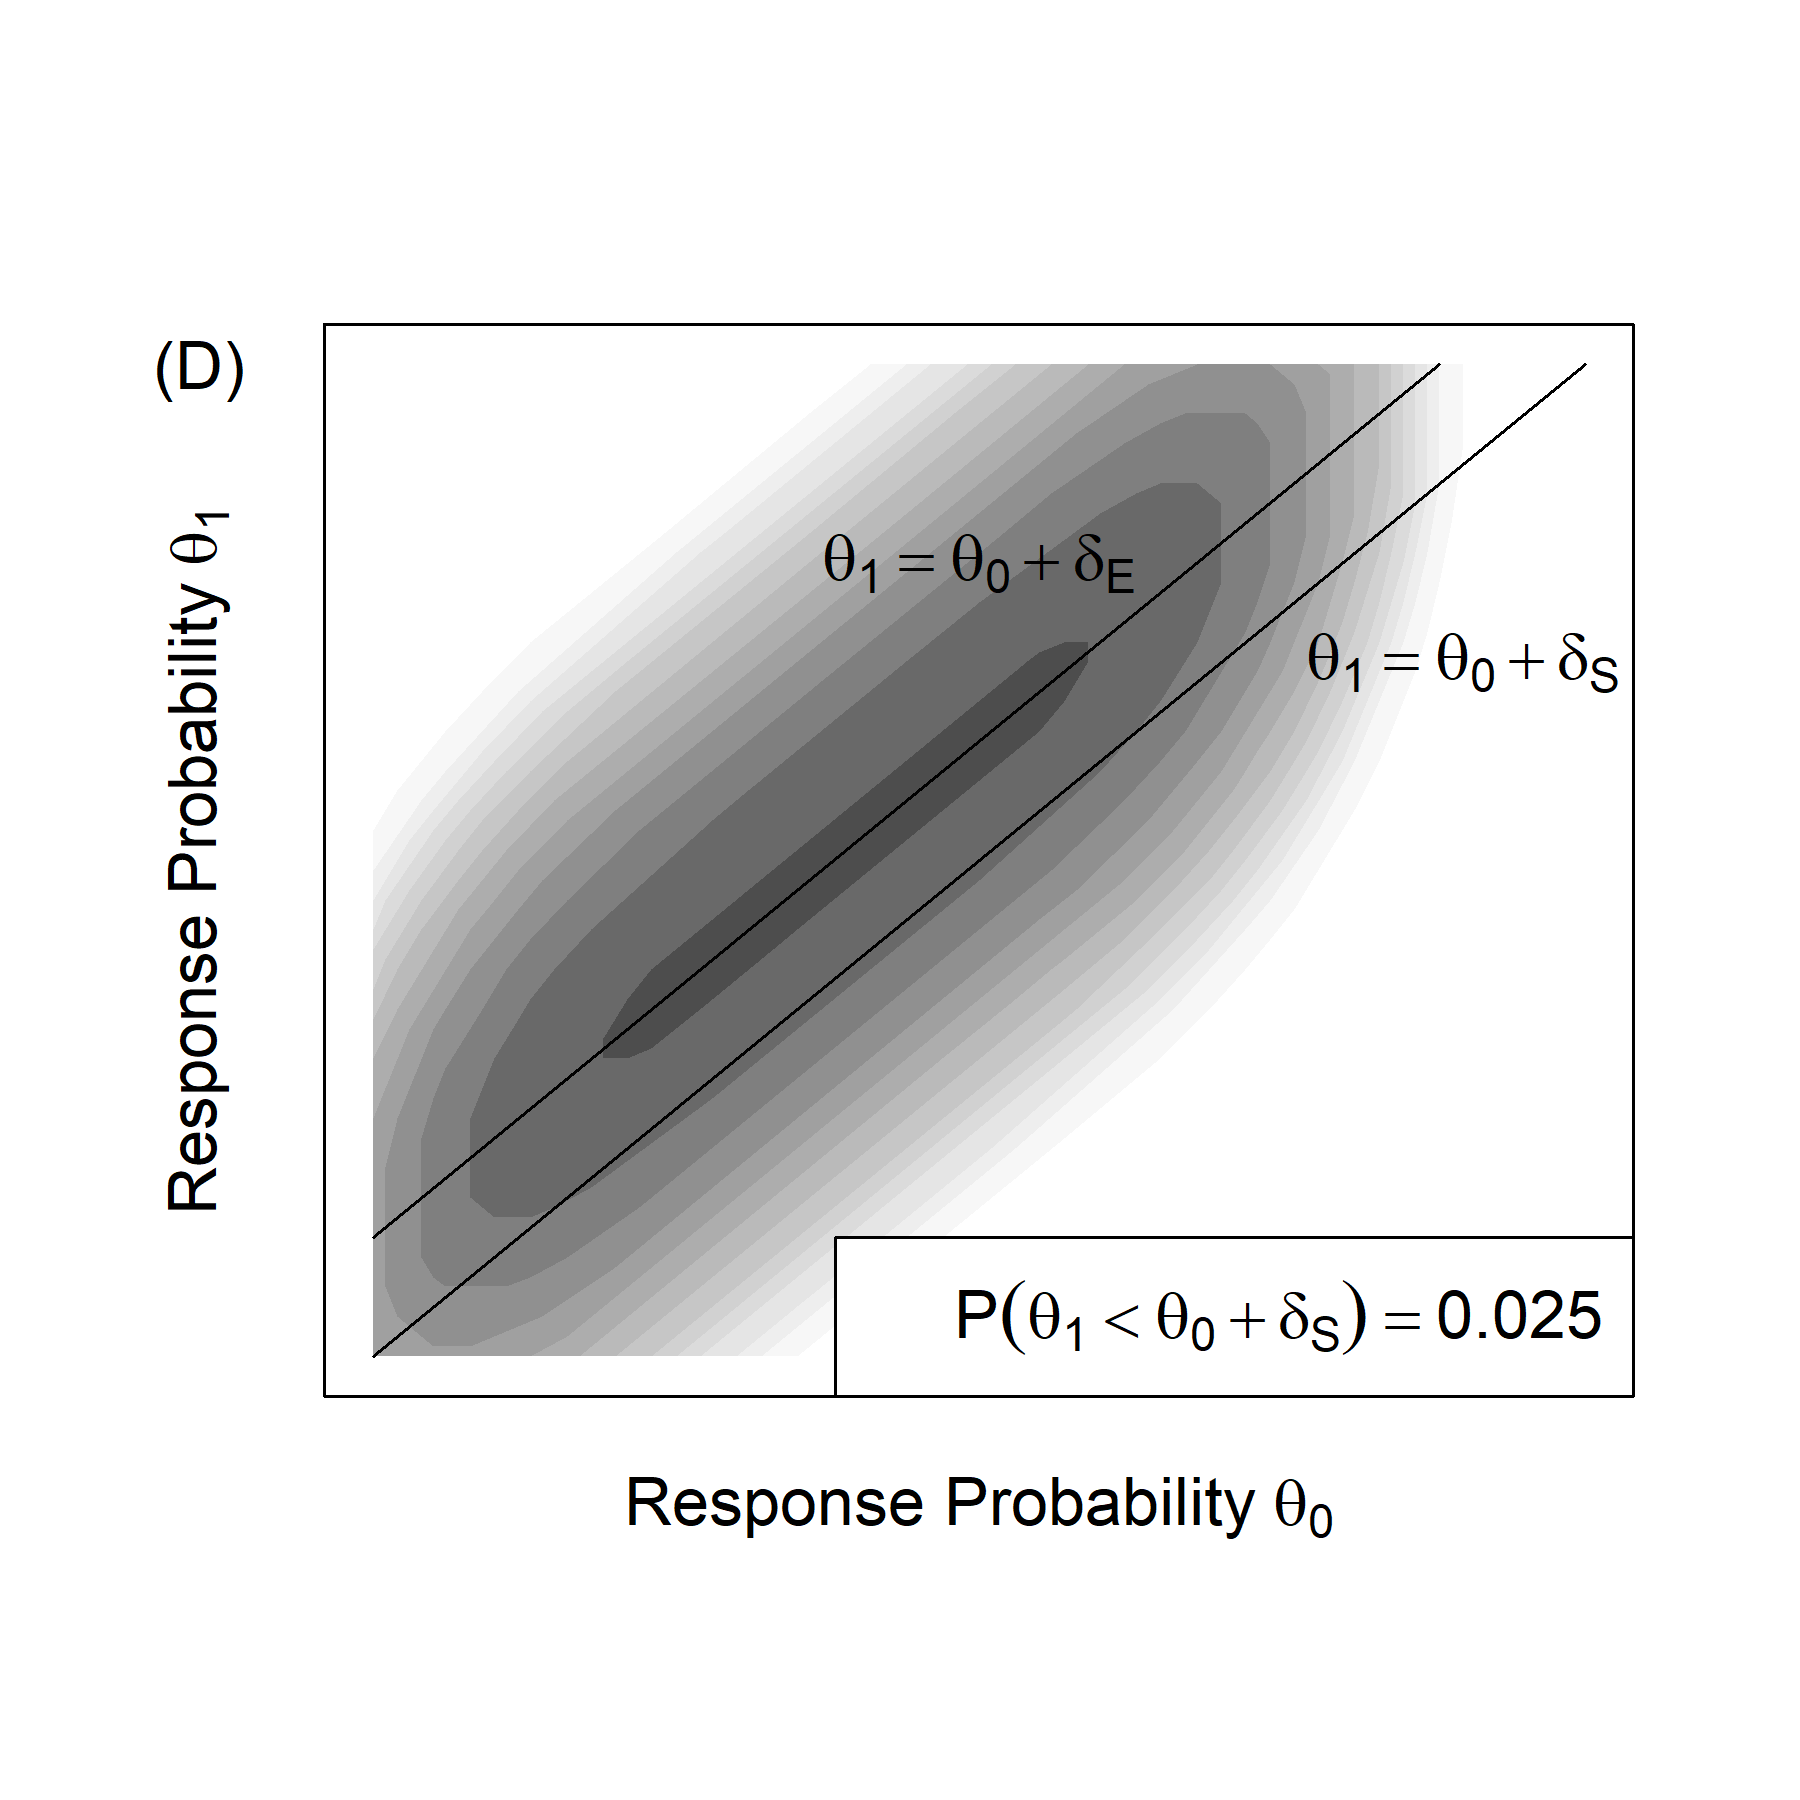
\includegraphics[scale=0.50]{./FIGURES/figure5b.png}
\text{Figure 5b: Skeptical prior on response difference in form of (\ref{eq:generalized_normal_IP}) $(\delta=0,\alpha_1=0.03,\beta_1=1.6)$}
    \end{center}	

		\begin{center}
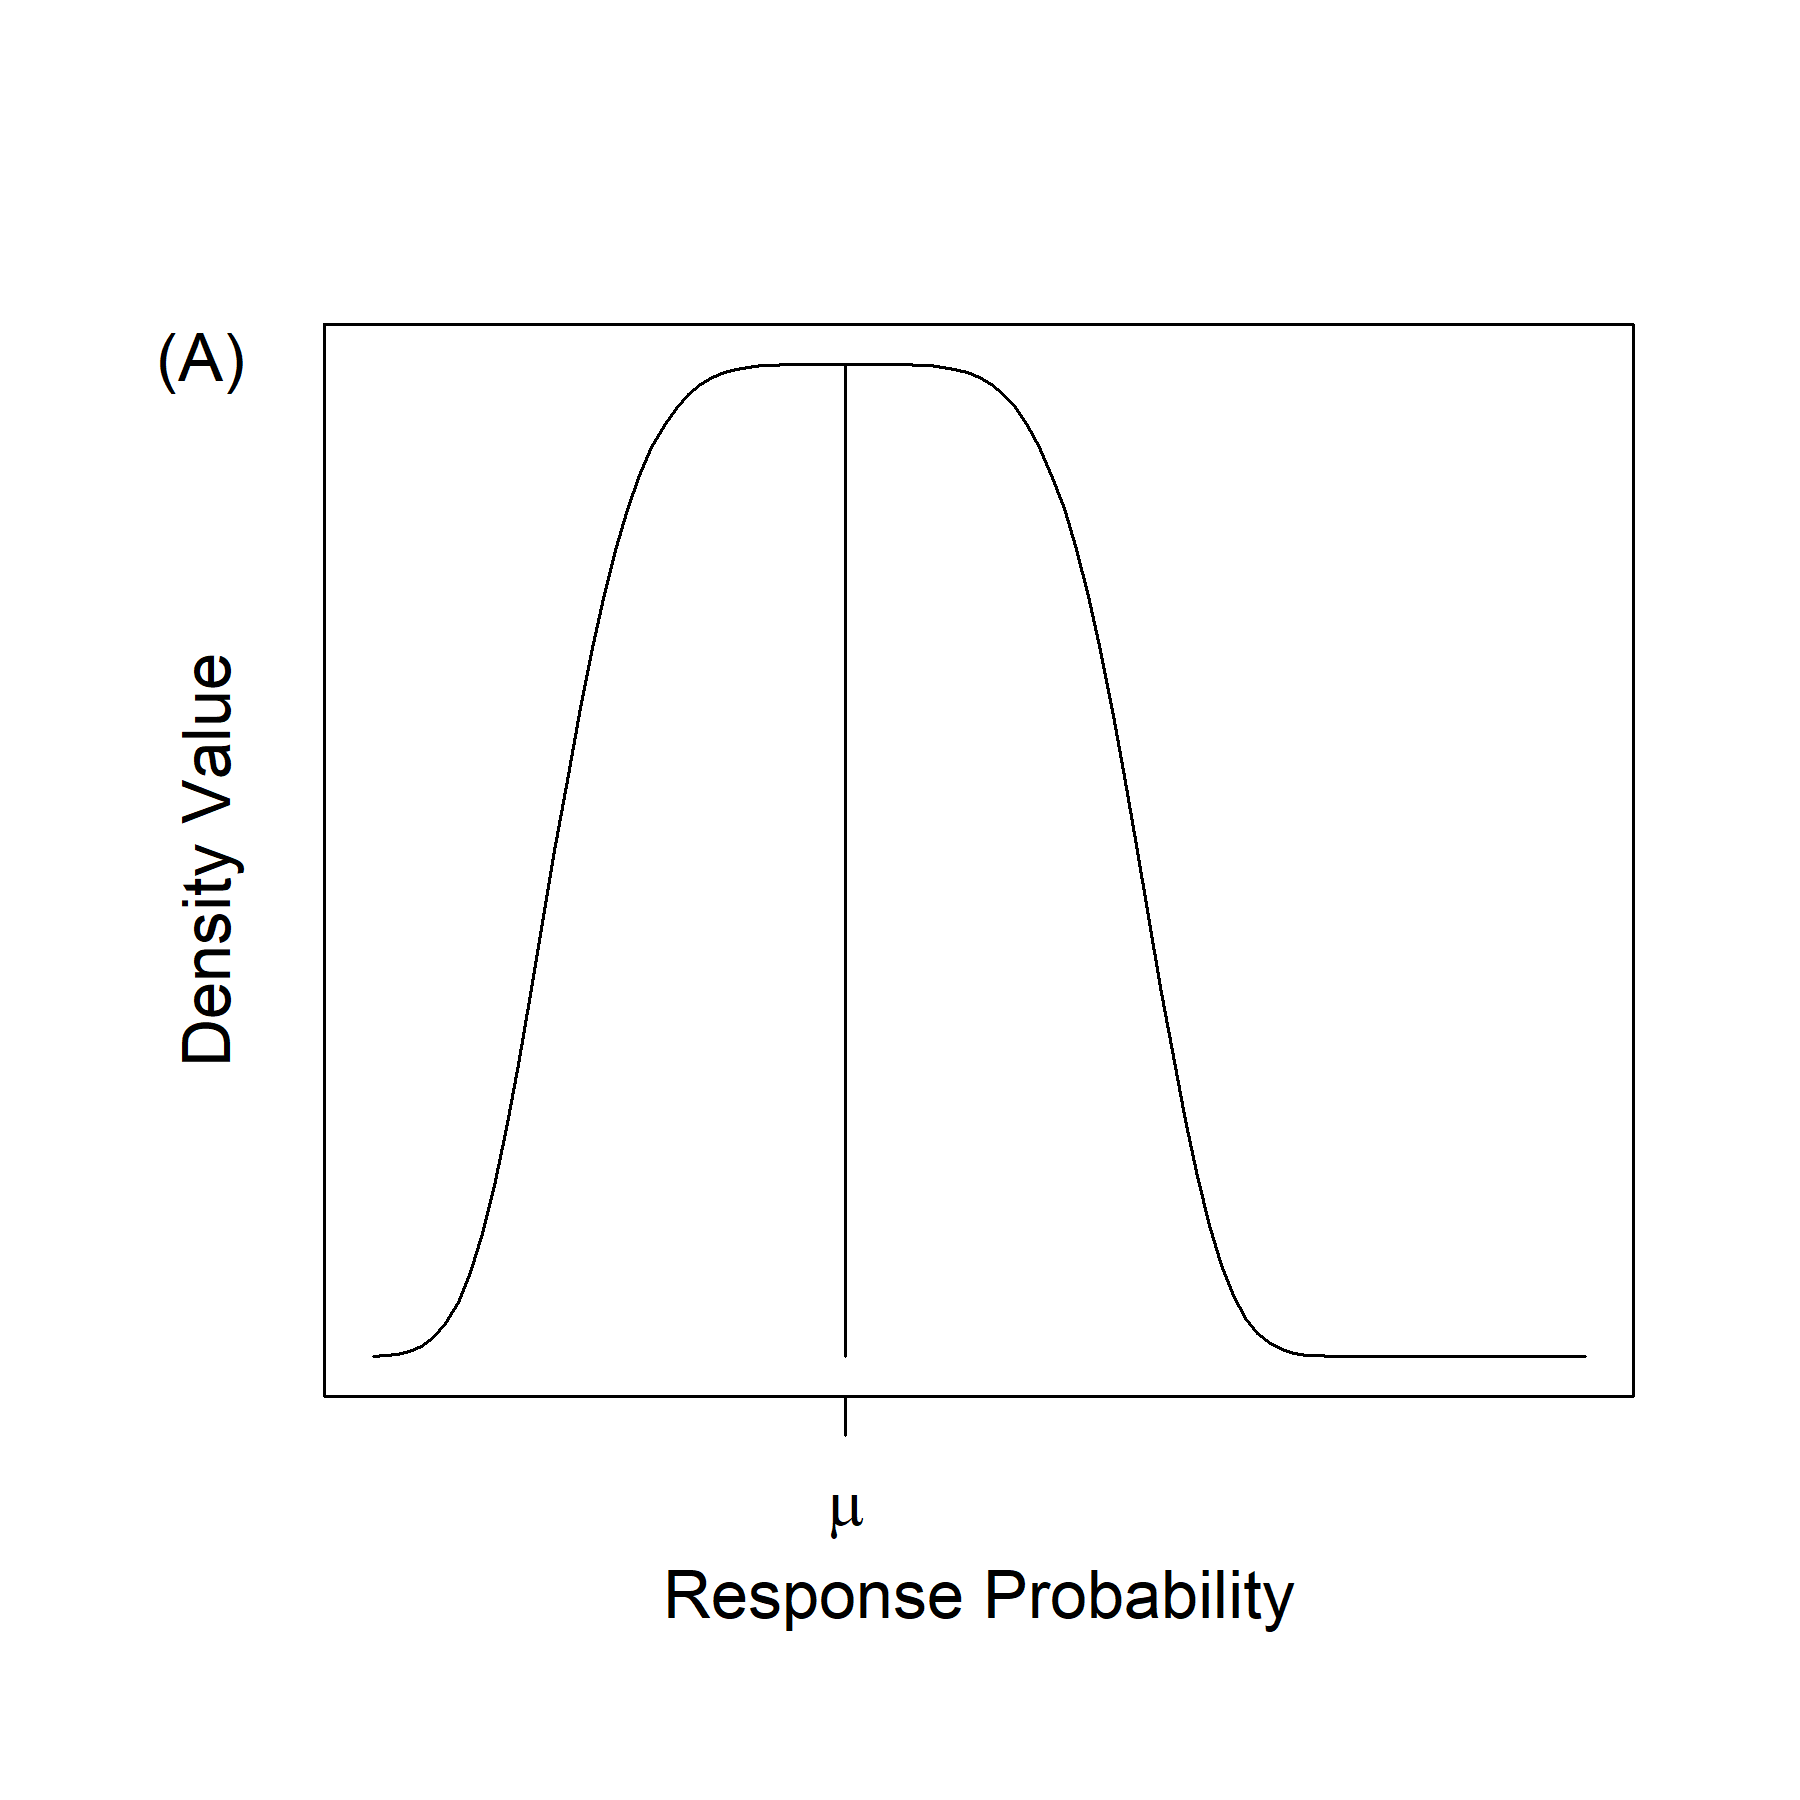
\includegraphics[scale=0.50]{./FIGURES/figure5c.png}

\text{Figure 5c: Enthuastic prior on response difference in form of (\ref{eq:generalized_normal_IP}) $(\delta=0.12,\alpha_1=0.087,\beta_1=2)$}
    \end{center}	

%\begin{align*}
%\pi(\theta_0,\theta_1)\propto& \hspace{0.05in}exp \left\{-\frac{1}{2}\left|\frac{(\theta_1-\theta_0)-\delta}{\sigma}\right|^\alpha\right\}
%\end{align*}





%Here we wish to elicit pessimistic and enthusiastic priors consistent with the following:
% \begin{enumerate}
%  \item The control group response probability is expected to be approximately $0.20$ and investigators are relatively sure
%		    that the it will be between 0.5 and 0.35.
%				
%	\item The IP group response probability is likely to provide an improvement of approximately 0.20.
%\end{enumerate}

Enrollment will proceed until one of the following three conditions are satisfied:
\begin{align*}
\text{Efficacy criteria (EFF): }&P(\theta_1-\theta_0>0|\mathbf{D},\pi_S)\geq 0.975\\
\text{Futility criteria (FUT): }&P(\theta_1-\theta_0 \leq 0.06|\mathbf{D},\pi_E)\geq 0.975\\
\text{Maximum sample size: }&N=100 \text{ patient outcomes}
\end{align*}

An interim analysis is compelted after every 10 subjects have completed outcomes.

%\begin{center}
%
%Table 1: Interim monitoring results (IP respones rate columns, PC response rate rows)
%
%\begin{tabular}{ll|ccccc}
%	&		&	0.05	&	0.1	&	0.15	&	0.2	&	0.25	\\
%\hline													
%0.05	&	EFF	&	0.12	&	0.72	&	0.97	&		&		\\
%	&	FUT	&	0.87	&	0.23	&	0.02	&		&		\\
%	&	SS initial	&	157	&	198	&	153	&		&		\\
%	&	SS final	&	173	&	213	&	169	&		&		\\
%\hline													
%0.1	&	EFF	&		&	0.18	&	0.60	&	0.92	&		\\
%	&	FUT	&		&	0.72	&	0.21	&	0.02	&		\\
%	&	SS initial	&		&	226	&	255	&	197	&		\\
%	&	SS final	&		&	240	&	268	&	212	&		\\
%\hline													
%0.15	&	EFF	&		&		&	0.14	&	0.53	&	0.82	\\
%	&	FUT	&		&		&	0.62	&	0.15	&	0.02	\\
%	&	SS initial	&		&		&	267	&	302	&	256	\\
%	&	SS final	&		&		&	279	&	311	&	269	\\
%\hline													
%										
%
%\end{tabular}
%
%
%
%\begin{tabular}{|c|}
%\hline
%EFF:$P(\theta_1-\theta_0>0|\textbf{D},\pi_S)\geq 0.95$\\
%\hline
%FUT:$P(\theta_1-\theta_0<0.05|\textbf{D},\pi_E)\geq 0.85$\\
%\hline
%\end{tabular}
%\end{center}

%\newpage
%\subsubsection{Example paths}
%\text{Stopping for efficacy:}
%\begin{center}
%\begin{tabular}{llll|cc}
%\multicolumn{2}{c}{Control}&\multicolumn{2}{c}{IP}&EFF&FUT\\
%\hline
%SS& $\hat{\theta}$ & SS & $\hat{\theta}$ &$P(\theta_1-\theta_0>0.1|\textbf{D},\pi_S(\theta_0,\theta_1))$&$P(\theta_1-\theta_0<0.15|\textbf{D},\pi_E(\theta_0,\theta_1))$\\
%\hline
%0&n/a&0&n/a& 0.401 &0.369\\
%5&0.2&5&0.6& 0.479 & 0.286\\
%10&0.2&10&0.6& 0.635 & 0.194\\
%15&0.2&15&0.6& 0.751 & 0.123\\
%20&0.2&20&0.6& 0.832 & 0.087\\
%25&0.2&25&0.6& 0.887 & 0.058\\
%30&0.2&30&0.6& 0.925 & 0.039\\
%35&0.2&35&0.6& 0.950 & 0.026
%\end{tabular}
%\end{center}
%\text{Stopping for futility:}
%\begin{center}
%\begin{tabular}{llll|cc}
%\multicolumn{2}{c}{Control}&\multicolumn{2}{c}{IP}&EFF&FUT\\
%\hline
%SS& $\hat{\theta}$ & SS & $\hat{\theta}$ &$P(\theta_1-\theta_0>0.1|\textbf{D},\pi_S(\theta_0,\theta_1))$&$P(\theta_1-\theta_0>0.15|\textbf{D},\pi_E(\theta_0,\theta_1))$\\
%\hline
%0&n/a&0&n/a& 0.401 &0.369\\
%5&0.4&5&0.4& 0.260 &0.527\\
%10&0.4&10&0.4& 0.236 & 0.613\\
%15&0.4&15&0.4& 0.219 & 0.681\\
%20&0.4&20&0.4& 0.203 & 0.735\\
%25&0.4&25&0.4& 0.189 & 0.778\\
%30&0.4&30&0.4& 0.175 & 0.813\\
%35&0.4&35&0.4& 0.163 & 0.842\\
%40&0.4&40&0.4& 0.151 & 0.866
%\end{tabular}
%\end{center}		
%\newpage

%Consider $\mu_0=0.50$, $\sigma_0=3.5$, $\sigma_1=7$, $\alpha_0=40$, $\alpha_1=30$, $\delta=0$.




      %\text{Prior for Control Group Response Probability \label{fig:pmp}}


\subsubsection{Design properties: Results}
%\subsection{Three-Arm, Placebo Controlled Non-Inferiority Trial w/ Continuous Endpoint}
%\begin{align*}
%P&\rightarrow\beta_0 \text{ (placebo)}\\
%C&\rightarrow\beta_0+\beta_1 \text{ (control)}\\
%A&\rightarrow\beta_0+\beta_1+\beta_2 \text{ (active)}\\
%H_0&:\beta_2-\delta\beta_1\leq 0
%\end{align*}
%Parameters of interest $(\beta_1,\beta_2)$, nuisance parameters $(\beta_0,\sigma^2)$.
%
%Need priors $\pi(\beta_0), \pi(\beta_1), \pi(\beta_2|\beta_1)$. 
%
%Will use MCMC to evaluate posteriors.

Simulations were run fixing the placebo response rate at $\theta_0=0.39$ and varying the treatment response rate $\theta_1\in[0.39,0.51]$. Due to the low maximum sample size, no simulations resulted in the efficacy criteria $(P(\theta_1-\theta_0>0|\mathbf{D},\pi_S)\geq 0.975)$ being satisfied. Instead of the skeptical prior $\pi_S$ being used for the efficacy critera, an inference prior $\pi_I$ of the form (\ref{eq:inference_prior}) is used where the choice of $\omega$ in (\ref{eq:omega_formula}) is determined based on varying $p(\pi_S)$ and $p(\pi_E)$ at the outset.
\begin{center}
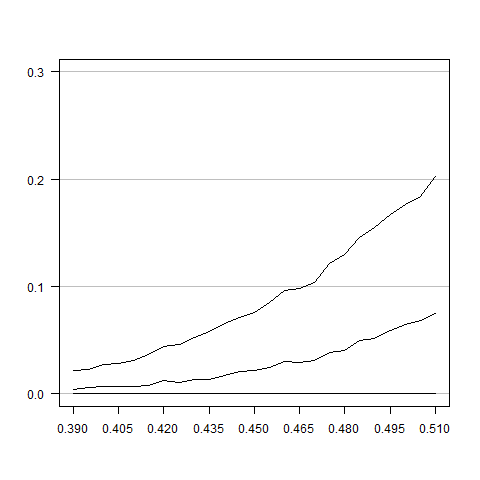
\includegraphics[width=5in]{P:/Git/Bayesian-Sequential-Monitoring/00-paper/FIGURES/figure6.png}

Figure 6: Probability of efficacy with three specifications of inference prior:\\
(1) $p(\pi_S)=1$, $p(\pi_E)=0$ (usual skeptical prior, lower line)\\
(2) $p(\pi_S)=0.75$, $p(\pi_E)=0.25$ (middle line)\\
(3) $p(\pi_S)=p(\pi_E)=0.5$ (upper line)
\end{center}
\section{Discussion}
%Q: Why not reverse engineer priors to have exact Type 1 error properties?
%
%A: This would basically be a frequentist method, in that the design would have to be adhered to exactly (including number and timing of data monitoring). Philosophically, designing a Bayesian study that requires rigid monitoring rules loses the advantages of Bayes from the likelihood principle.




\section{Supplementary material}


\subsubsection{Type 1 error rate depending on enrollment schemes}
Consider the same trial but with a longer follow-up length of 8 months rather than 4 months. 
\begin{center}
Table 2: Comparison of efficacy stopping, Type 1 Error Rate (efficacy criteria with full data), and sample size by follow-up length and frequency of sequential monitoring.
\begin{tabular}{l | cccc|cccc}
	&	4 month FU	&		&		&		&	8 month FU	&		&		&		\\
															
\# Monitoring Freq	&	EFF	&	T1E	&	SS Final	&	Ongoing	&	EFF	&	T1E	&	SS Final	&	Ongoing	\\
\hline		
1&0.046&0.018& 77.1& 8.1\%&0.045&0.014& 94.0&24.6\%\\
2&0.039&0.018& 79.2& 7.7\%&0.039&0.014& 95.4&23.4\%\\
3&0.037&0.019& 79.9& 7.5\%&0.038&0.014& 96.0&22.8\%\\
5&0.034&0.017& 82.2& 7.2\%&0.035&0.014& 97.3&22.1\%\\
10&0.030&0.019& 85.3& 6.7\%&0.030&0.013& 99.5&19.8\%\\
20&0.024&0.017& 90.6& 5.9\%&0.021&0.012&102.7&17.2\%\\
61&0.019&0.015& 98.3& 2.6\%&0.019&0.014&106.3& 9.8\%\\
112&0.012&0.012&112.0& 0.0\%&0.012&0.012&112.0& 0.0\%\\
\end{tabular}
\end{center}
Monitoring Freq is 1 for fully sequential design and 112 when the only analysis is with all completed outcomes.

Note that the probability of efficacy stopping and Type 1 error rate increase monotonically for both specifications of follow-up length. The Type 1 error rate is lower for the 8-month follow-up design since there are more subjects in the final sample size.
%\begin{figure}
%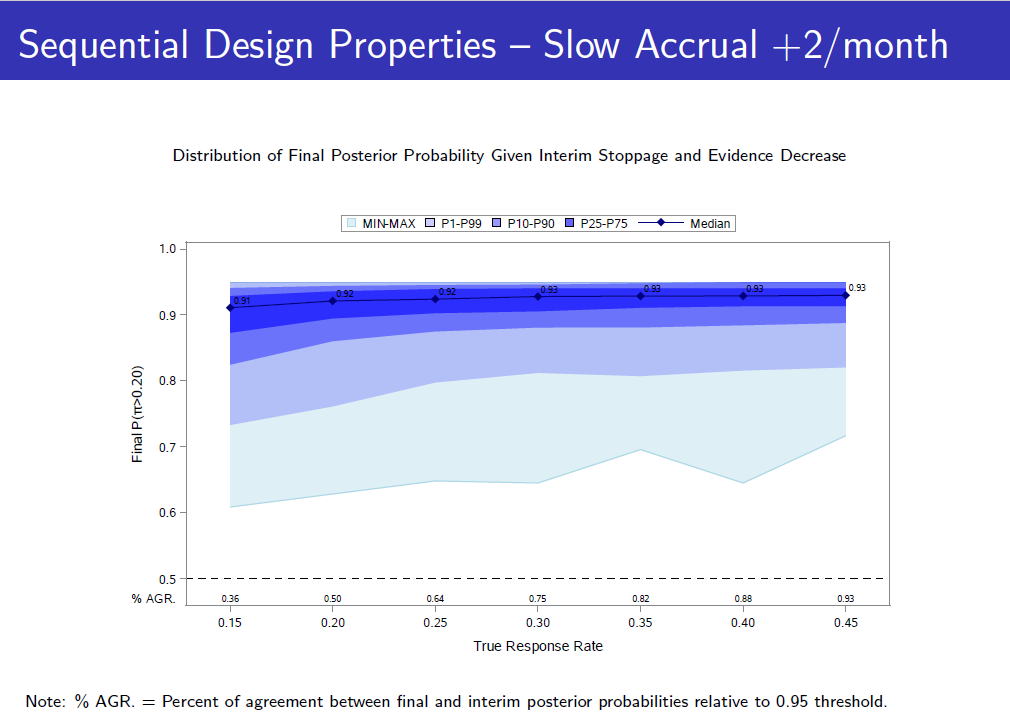
\includegraphics[width=6in]{P:/Git/Bayesian-Sequential-Monitoring/00-paper/FIGURES/evidence_decrease.png}
%\caption{Have the necessary data summaries in R, just need to replicate the plot.}
%\end{figure}

%The inference priors will be of the form $\pi_{I}=\omega\cdot\pi_{S}+(1-\omega)\cdot\pi_E$ with $\omega\in\{0,1/4,1/2,3/4,1\}$.
%\begin{center}
%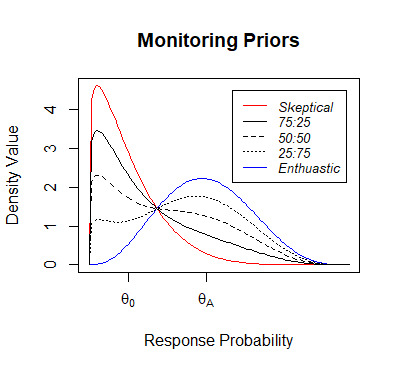
\includegraphics[width=5in]{P:/Git/Bayesian-Sequential-Monitoring/00-paper/FIGURES/figure3_2.png}
%\end{center}

%\begin{center}
%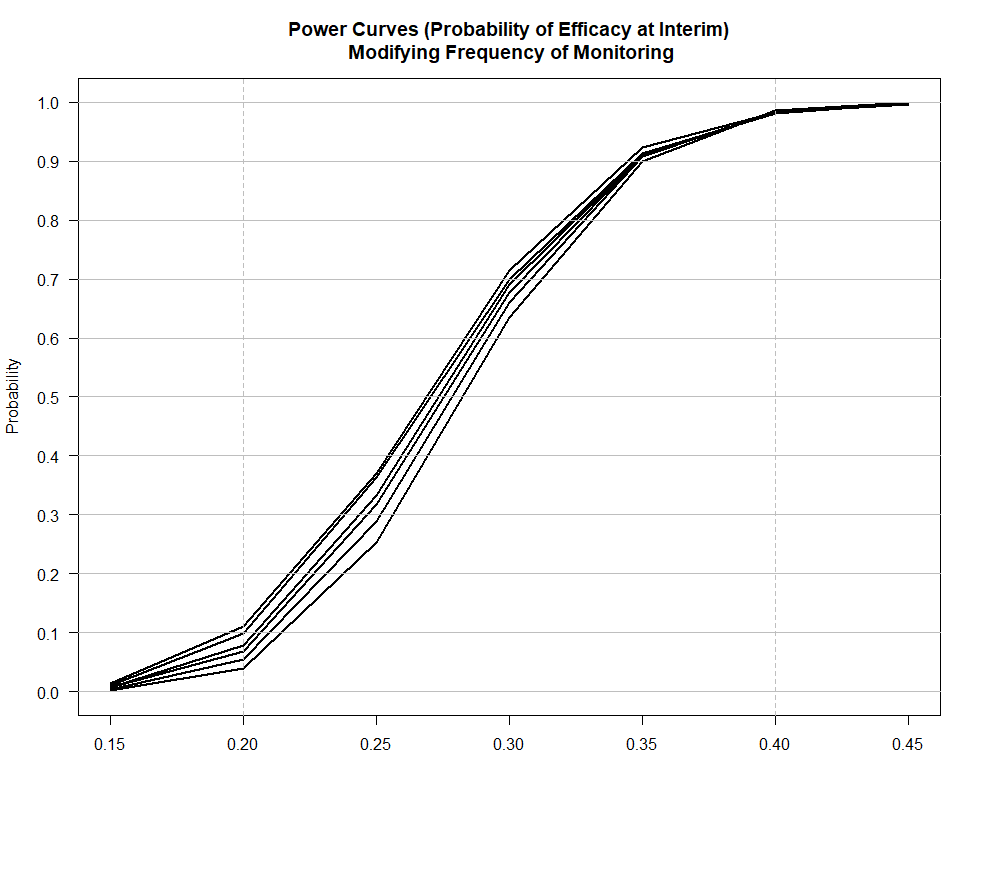
\includegraphics[width=3in]{P:/Git/Bayesian-Sequential-Monitoring/00-paper/FIGURES/power_curves}
%\end{center}
\newpage
\subsubsection{Robustness of parameterizations of monitoring priors}
%The generalized normal distribution is used to create priors with the same expected value and tail area as the default beta priors, but with densities that are either spike/slab around the expected value or flattened.
%\begin{figure}
%\begin{center}
%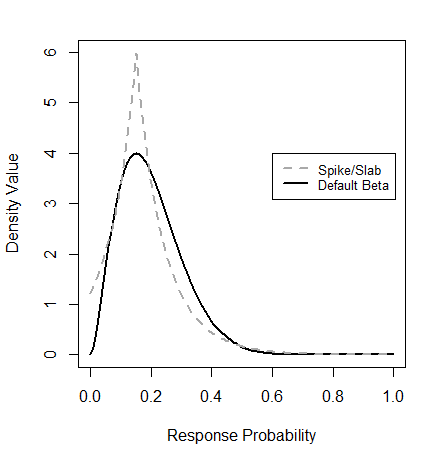
\includegraphics[width=3.5in]{P:/Git/Bayesian-Sequential-Monitoring/00-paper/FIGURES/spike-slab_skeptical}
%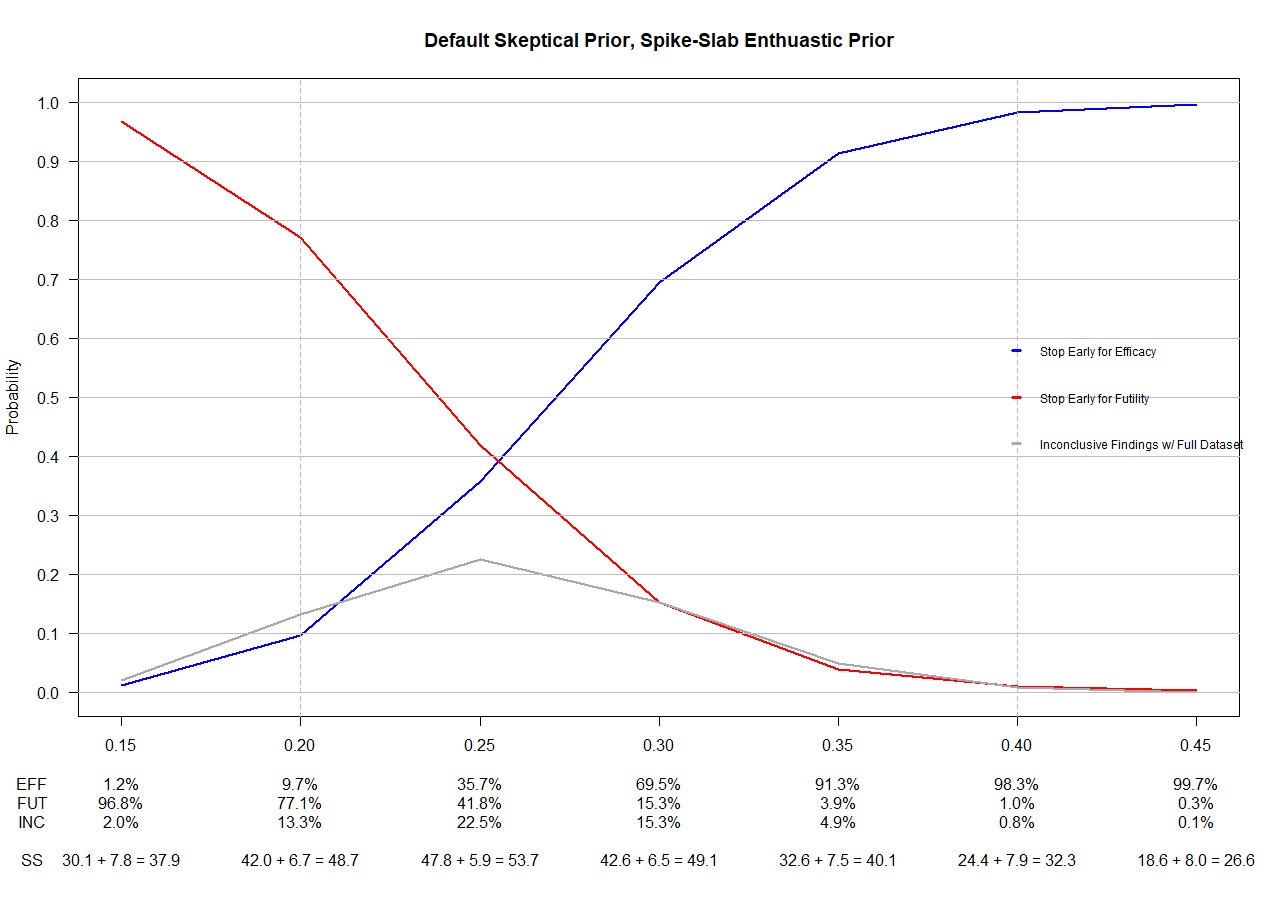
\includegraphics[width=3.5in]{P:/Git/Bayesian-Sequential-Monitoring/00-paper/FIGURES/spike-slab_enthuastic}
%% \caption{(a) Skeptical priors (b) Enthuastic priors}
%%\end{figure}
%
%Figure 6: (a) Alternate skeptical priors (b) Alternate enthuastic priors
%\end{center}
Model "1" corresponds to default skeptical and enthuasic priors, "2" is concentrated skeptical and default enthuastic (the case considered in the main text), "3" is default skeptical and flattened enthaustic, and "4" is concentrated skeptical and flattened enthaustic.
\begin{center}
\text{Table 3: Sequential design properties using alternative monitoring priors}
\begin{tabular}{ll|ccccc}
&&0.4&0.4675&0.535&0.6025&0.67\\
\hline
1&EFF&0.073&0.418&0.869&0.993&1.000\\
1&FUT&0.755&0.255&0.026&0.001&0.000\\
1&INC&0.172&0.326&0.105&0.005&0.000\\
1&SS&71.0 + 6.3 = 77.3&79.3 + 5.1 = 84.4&56.9 + 7.0 = 63.9&34.4 + 8.0 = 42.4&23.0 + 8.0 = 31.0\\
\hline
2&EFF&0.039&0.313&0.805&0.988&1.000\\
2&FUT&0.765&0.252&0.026&0.001&0.000\\
2&INC&0.196&0.435&0.169&0.011&0.000\\
2&SS&72.9 + 6.2 = 79.1&87.5 + 4.1 = 91.7&67.1 + 6.3 = 73.5&41.4 + 7.8 = 49.3&27.7 + 8.0 = 35.7\\
\hline
3&EFF&0.071&0.415&0.871&0.994&1.000\\
3&FUT&0.811&0.314&0.036&0.001&0.000\\
3&INC&0.118&0.271&0.093&0.005&0.000\\
3&SS&66.5 + 6.8 = 73.4&76.6 + 5.5 = 82.1&56.3 + 7.1 = 63.3&34.5 + 8.0 = 42.5&23.0 + 8.0 = 31.0\\
\hline
4&EFF&0.040&0.313&0.803&0.987&1.000\\
4&FUT&0.815&0.321&0.038&0.002&0.000\\
4&INC&0.144&0.366&0.159&0.011&0.000\\
4&SS&68.8 + 6.7 = 75.5&84.1 + 4.7 = 88.9&66.5 + 6.5 = 72.9&41.9 + 7.9 = 49.8&27.7 + 8.0 = 35.7\\

\end{tabular}
\end{center}
%Use of a spike-slab skeptical prior drastically lowers the probability of terminating enrollment due to efficacy, from $0.094$ in the default case to $0.066$. This is because there is less probability mass in the immediate area greater than the null value of $0.2$. When using a flattened skeptical prior the probability of terminating enrollment due to efficacy increases to $0.142$ since there is more probability mass in the immediate area greater than the null value of $0.2$.
%\bigskip
%\newpage
%\begin{center}
%{\large\bf SUPPLEMENTARY MATERIAL}
%\end{center}
%\section{Beta Priors}
%Beta priors for $\theta$ will be used to provide closed-form expressions of the posterior distributions via Beta-Binomial conjugacy (the posterior distribution $p(\theta|\mathbf{D})$ will be Beta distributed). The Beta distribution has two shape parameters. These parameters can be determined uniquely by specifying the desired mean and variance of the distribution.  The variance for the skeptical and enthuastic priors is then uniquely determined through by the choice of threshold $\delta$. In particular, let $\pi_S(\theta)\sim \mathcal{B}(\alpha,\beta)$ be Beta distributed with shape parameters $(\alpha,\beta)$. There is a single choice of $(\alpha,\beta)$ such that:
%\begin{align*}
%\theta_0=E(\pi_S)=\int_{\Theta}\pi_S(\theta)d\theta=\frac{\alpha}{\alpha+\beta}\text{ and }\delta=\int_{\Theta_0}\pi_S(\theta)d\theta=\int_{0}^{\theta_0}\frac{\theta^{\alpha-1}(1-\theta)^{\beta-1}}{B(\alpha,\beta)}d\theta
%\end{align*}
%where $B(\alpha,\beta)$ is the Beta function.
%
%Alternatively, the variance could be determined by specifying a desired quantile of the prior distribution which would then be reflected in $\delta$.  Then there is a single choice of $(\alpha,\beta)$ such that
%\begin{align*}
%\theta_0=E(\pi_S)=\int_{\Theta}\pi_S(\theta)d\theta=\frac{\alpha}{\alpha+\beta}\text{ and }\lambda=\int_{\theta_A}^{1}\pi_S(\theta)d\theta=\int_{\theta_A}^{1}\frac{\theta^{\alpha-1}(1-\theta)^{\beta-1}}{B(\alpha,\beta)}d\theta,
%\end{align*}
%in which case $\delta=\int_{\Theta_0}\pi_S(\theta)d\theta$ is a deterministic quantity.
%\begin{center}
%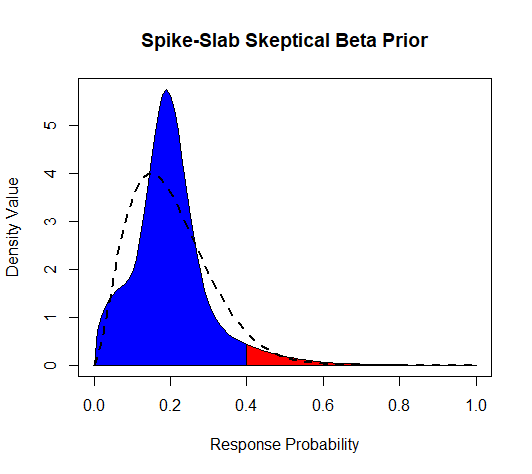
\includegraphics[width=5in]{P:/Git/Bayesian-Sequential-Monitoring/00-paper/FIGURES/ss_skpt}
%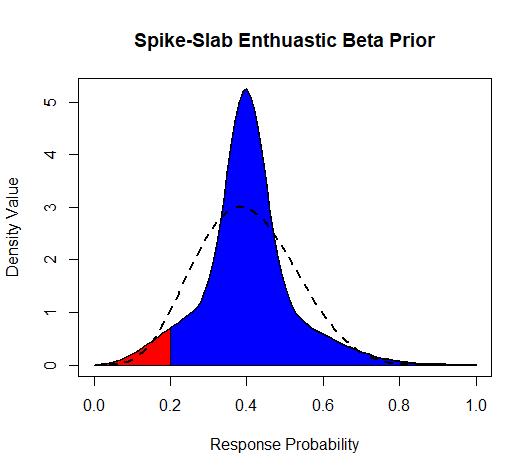
\includegraphics[width=5in]{P:/Git/Bayesian-Sequential-Monitoring/00-paper/FIGURES/ss_enth}
%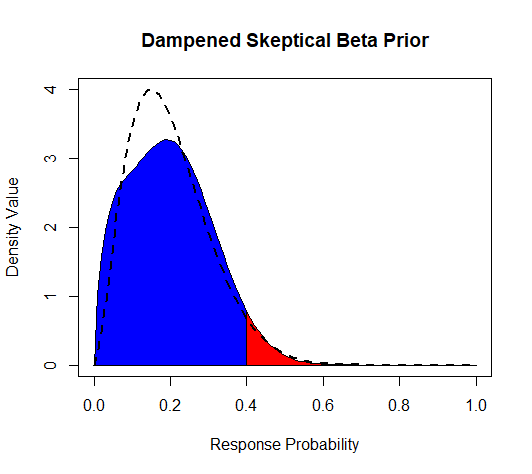
\includegraphics[width=5in]{P:/Git/Bayesian-Sequential-Monitoring/00-paper/FIGURES/damp_skpt}
%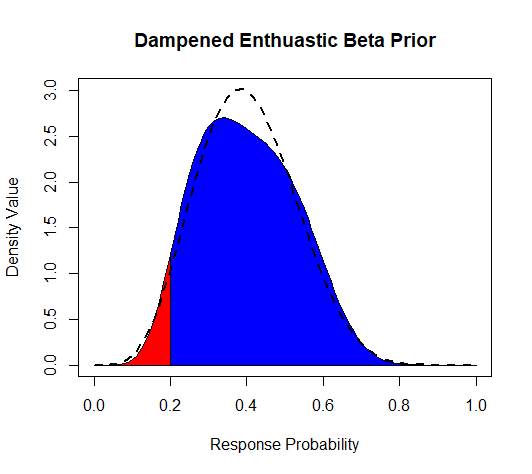
\includegraphics[width=5in]{P:/Git/Bayesian-Sequential-Monitoring/00-paper/FIGURES/damp_enth}
%\end{center}
\section{BibTeX}

 \bibliographystyle{agsm}
 \bibliography{./References}		

\end{document}
